\documentclass[11pt]{article}

\usepackage[utf8]{inputenc}
\pagenumbering{arabic}
\usepackage[centertags]{amsmath}
\usepackage{amssymb}
\usepackage{mathrsfs}
\usepackage[usenames]{color}
\usepackage{enumerate}
\usepackage{graphicx}
\usepackage[english]{babel}
\usepackage{setspace}
\usepackage{float}
\usepackage{subfig}
\usepackage{hyperref}
\usepackage{booktabs}
\usepackage[left=1.25in,right=1in,top=1.25in,bottom=1.25in]{geometry}

\graphicspath{{./}}

\newcommand{\bs}{\boldsymbol}
\newcommand{\pa}{\partial}

\parskip=6pt
\parindent=0mm
\singlespacing

\title{\textsc{\textbf{OASIS}} \\ \textsc{Offshore Advanced Simulation Software} \\ \textsc{---} \\ \textsc{Theory Manual}}
\author{\'Alvaro Rodr\'iguez Luis}
\date{April 2026}

\begin{document}

\maketitle
\vfill
\begin{figure}[H]
\centering
\captionsetup[subfigure]{labelformat=empty}
\subfloat[]{
\includegraphics[width=0.3\columnwidth]{logo.jpg}}
\hspace{1cm}
\subfloat[]{
\includegraphics[width=0.3\columnwidth]{logo.png}}
\end{figure}
\begin{center}
\textbf{Offshore Engineering and Ocean Energy Group}\\
\textbf{Environmental Hydraulics Institute of Cantabria}
\end{center}
\vfill
\clearpage

\tableofcontents
\clearpage

%%%%%%%%%%%%%%%%%%%%%%%%%%%%%%%%%%%%%%%%%%%%%%%%%%%%%%%%%%%%
\section{Introduction}
%%%%%%%%%%%%%%%%%%%%%%%%%%%%%%%%%%%%%%%%%%%%%%%%%%%%%%%%%%%%

OASIS (Offshore Advanced Simulation Software) is a time-domain numerical simulation tool for offshore floating structures developed in C++ at IHCantabria. It couples potential-flow hydrodynamics with structural and mooring dynamics to predict the motion response of floating platforms under waves, wind and current.

The software is structured as a collection of coupled modules, each solving a specific physical subsystem. The modules are:

\begin{itemize}
    \item \textbf{Rigid body dynamics} --- six degree-of-freedom (6-DOF) motion of floating bodies.
    \item \textbf{Waves} --- generation of regular and irregular sea states.
    \item \textbf{Hydrostatics} --- linear restoring forces and non-linear Froude--Krylov pressure integration.
    \item \textbf{Hydrodynamics} --- potential-flow radiation/diffraction framework including first- and second-order wave loads, Morison drag for wind and current.
    \item \textbf{Mooring and towing lines} --- spectral element method (SEM) formulation for dynamic cable simulation.
    \item \textbf{Seafloor interaction} --- seabed projection algorithms for flat, inclined and complex bathymetries.
    \item \textbf{Springs and connectors} --- 6-DOF spring/damper/friction model for multi-body coupling.
    \item \textbf{Winches} --- mechanical winch model with controllers.
    \item \textbf{Oscillating water columns (OWC)} --- pneumatic chamber and turbine model.
    \item \textbf{Wind turbines} --- coupling interface to OpenFAST.
    \item \textbf{Sinking} --- progressive flooding model with time-varying hydrostatic and hydrodynamic properties.
\end{itemize}

All subsystems are assembled into a single initial value problem (IVP) and integrated in time using implicit ODE solvers (BDF2 or ESDIRK) with adaptive step-size control. The coupling among subsystems is described in Section~\ref{sec:coupling}.

This document describes the mathematical formulation behind each module and how they are coupled together. References to the corresponding source code files are given throughout.

%%%%%%%%%%%%%%%%%%%%%%%%%%%%%%%%%%%%%%%%%%%%%%%%%%%%%%%%%%%%
\section{Coordinate Systems and Rigid Body Dynamics}
\label{sec:bodies}
%%%%%%%%%%%%%%%%%%%%%%%%%%%%%%%%%%%%%%%%%%%%%%%%%%%%%%%%%%%%

\subsection{Reference frames}

Two types of reference frames are used:

\begin{enumerate}
    \item \textbf{Global inertial frame}: a fixed reference frame with its origin at the mean free surface. The first two basis vectors ($\mathbf{e}_1$, $\mathbf{e}_2$) are tangent to the undisturbed water surface, and $\mathbf{e}_3$ points upward.
    \item \textbf{Local body frame}: a non-inertial frame with its origin at the centre of gravity (COG) of each body. When the body is at rest, the local axes coincide with the global axes. The frame moves with the body.
\end{enumerate}

\subsection{Euler angles and rotation matrices}

Body rotations are described using Tait--Bryan (nautical) angles: roll ($\alpha$), pitch ($\beta$) and yaw ($\gamma$). These define three successive rotations around the global axes $X$, $Y$ and $Z$:

\begin{equation}
\mathbf{R}_1(\alpha) = \begin{pmatrix} 1 & 0 & 0 \\ 0 & \cos\alpha & -\sin\alpha \\ 0 & \sin\alpha & \cos\alpha \end{pmatrix}, \quad
\mathbf{R}_2(\beta) = \begin{pmatrix} \cos\beta & 0 & \sin\beta \\ 0 & 1 & 0 \\ -\sin\beta & 0 & \cos\beta \end{pmatrix}, \quad
\mathbf{R}_3(\gamma) = \begin{pmatrix} \cos\gamma & -\sin\gamma & 0 \\ \sin\gamma & \cos\gamma & 0 \\ 0 & 0 & 1 \end{pmatrix}
\end{equation}

The combined rotation matrix is $\mathbf{R}(\alpha,\beta,\gamma) = \mathbf{R}_3(\gamma)\cdot\mathbf{R}_2(\beta)\cdot\mathbf{R}_1(\alpha)$.

The position of the body is defined by:
\begin{equation}
\mathbf{r} = \begin{pmatrix} x \\ y \\ z \end{pmatrix}, \quad \boldsymbol{\Phi} = \begin{pmatrix} \alpha \\ \beta \\ \gamma \end{pmatrix}
\end{equation}

where $\mathbf{r}$ contains the COG coordinates in the global frame and $\boldsymbol{\Phi}$ the Euler angles. A point with local coordinates $\mathbf{p}_L$ has global coordinates:
\begin{equation}
\mathbf{p}_G = \mathbf{r} + \mathbf{R}(\boldsymbol{\Phi})\cdot\mathbf{p}_L
\end{equation}

Its velocity and acceleration in the global frame are:
\begin{equation}
\dot{\mathbf{p}}_G = \dot{\mathbf{r}} + \dot{\mathbf{R}}(\boldsymbol{\Phi},\dot{\boldsymbol{\Phi}})\cdot\mathbf{p}_L, \qquad \ddot{\mathbf{p}}_G = \ddot{\mathbf{r}} + \ddot{\mathbf{R}}(\boldsymbol{\Phi},\dot{\boldsymbol{\Phi}},\ddot{\boldsymbol{\Phi}})\cdot\mathbf{p}_L
\end{equation}

\subsection{Newton--Euler equations for the rigid body}

Forces and moments can be computed at the COG or at arbitrary body points. A force $\mathbf{F}$ and moment $\mathbf{M}$ applied at a body point with local coordinates $\mathbf{p}_L$ produce equivalent quantities at the COG:
\begin{equation}
\mathbf{F}_{\text{cm}} = \mathbf{F}, \qquad \mathbf{M}_{\text{cm}} = \mathbf{M} + \mathbf{p}_L \times \left(\mathbf{R}^T(\boldsymbol{\Phi})\cdot\mathbf{F}\right)
\end{equation}

The net forces $\sum\mathbf{F}_{\text{cm},i}$ and moments $\sum\mathbf{M}_{\text{cm},i}$ at the COG are assembled from all acting subsystems (hydrodynamics, mooring lines, springs, wind turbines, OWC, etc.). The body accelerations are obtained from:
\begin{equation}
\left[\begin{pmatrix} m\cdot\mathbf{I}_{3\times 3} & \mathbf{0}_{3\times 3} \\ \mathbf{0}_{3\times 3} & \mathbf{I}_b \end{pmatrix} + \mathbf{A}\right] \cdot \begin{pmatrix} \ddot{\mathbf{r}} \\ \ddot{\boldsymbol{\Phi}} \end{pmatrix} = \begin{pmatrix} \sum\mathbf{F}_{\text{cm},i} \\ \sum\mathbf{M}_{\text{cm},i} \end{pmatrix}
\label{eq:newton}
\end{equation}

where $m$ is the structural mass, $\mathbf{I}_b$ is the inertia matrix in the principal body axes, and $\mathbf{A}$ is the added mass matrix (at infinite frequency) plus any viscous added mass corrections:
\begin{equation}
\mathbf{A} = \mathbf{A}_\infty + \mathbf{A}_{\text{visc}}
\end{equation}

For multi-body systems, the matrices are assembled in block-diagonal form, with off-diagonal coupling through the hydrodynamic added mass.

%%%%%%%%%%%%%%%%%%%%%%%%%%%%%%%%%%%%%%%%%%%%%%%%%%%%%%%%%%%%
\section{Waves}
\label{sec:waves}
%%%%%%%%%%%%%%%%%%%%%%%%%%%%%%%%%%%%%%%%%%%%%%%%%%%%%%%%%%%%

\subsection{Regular waves}

A regular wave is described by a single component with height $H$, period $T$ and heading $\varphi$. The free surface elevation at position $(x,y)$ and time $t$ is:
\begin{equation}
\eta(x,y,t) = \frac{H}{2}\cos\left(k_x x + k_y y - \omega t + \phi_0\right) \cdot r(t)
\end{equation}

where $\omega = 2\pi/T$ is the angular frequency, $k_x = k\cos\varphi$, $k_y = k\sin\varphi$, $\phi_0$ is the initial phase, and $r(t)$ is a ramp function for smooth startup. The wavenumber $k$ is obtained from the linear dispersion relation:
\begin{equation}
\omega^2 = g\,k\tanh(k\,h)
\end{equation}
solved iteratively using Newton--Raphson's method, where $g$ is gravitational acceleration and $h$ is water depth.

\subsection{Irregular waves (JONSWAP)}

Irregular sea states are represented as a superposition of $n_C$ wave components:
\begin{equation}
\eta(x,y,t) = \sum_{i=1}^{n_C}\sum_{j=1}^{n_H} a_{ij}\cos\left(k_{x,i}\cos\varphi_j\, x + k_{y,i}\sin\varphi_j\, y - \omega_i t + \phi_{ij}\right)\cdot r(t)
\end{equation}

where $a_{ij} = \sqrt{2\,S(\omega_i)\,D(\varphi_j)\,\Delta\omega\,\Delta\varphi}$ is the amplitude from the directional spectrum.

The JONSWAP spectrum is defined as:
\begin{equation}
S(\omega) = \frac{\alpha g^2}{\omega^5}\exp\left[-\frac{5}{4}\left(\frac{\omega_p}{\omega}\right)^4\right]\gamma^{\exp\left[-\frac{(\omega-\omega_p)^2}{2\sigma^2\omega_p^2}\right]}
\end{equation}

where $\omega_p = 2\pi/T_p$ is the peak frequency, $\gamma$ is the peak enhancement factor, $\sigma = 0.07$ for $\omega \leq \omega_p$ and $\sigma = 0.09$ for $\omega > \omega_p$, and $\alpha$ is chosen so that the zeroth spectral moment matches $H_s^2/16$.

\subsection{Directional spreading}

Directional spreading is modelled using the cosine-power function:
\begin{equation}
D(\varphi) = C_s\cos^{2s}\left(\frac{\varphi - \varphi_0}{2}\right)
\end{equation}
where $s$ is the spreading parameter and $C_s$ is a normalisation constant such that $\int D(\varphi)\,d\varphi = 1$.

The dynamic pressure at a point $(x,y,z)$ due to the wave field is computed using linear wave theory:
\begin{equation}
p(x,y,z,t) = \rho_w g \sum_{i=1}^{n_C} a_i\frac{\cosh[k_i(z+h)]}{\cosh(k_i h)}\cos(k_{x,i}x + k_{y,i}y - \omega_i t + \phi_i)
\end{equation}


%%%%%%%%%%%%%%%%%%%%%%%%%%%%%%%%%%%%%%%%%%%%%%%%%%%%%%%%%%%%
\section{Hydrostatics}
\label{sec:hydrostatics}
%%%%%%%%%%%%%%%%%%%%%%%%%%%%%%%%%%%%%%%%%%%%%%%%%%%%%%%%%%%%

\subsection{Linear hydrostatic restoring}

For small displacements from equilibrium, the hydrostatic restoring force is:
\begin{equation}
\mathbf{F}_{\text{hs}} = -\mathbf{G}\cdot\boldsymbol{\nu}
\end{equation}

where $\mathbf{G}$ is the $6\times 6$ hydrostatic stiffness matrix (computed from the equilibrium waterplane area, COG and centre of buoyancy) and $\boldsymbol{\nu} = (\mathbf{r}^T, \boldsymbol{\Phi}^T)^T$ is the 6-DOF displacement vector.

\subsection{Non-linear Froude--Krylov}

For large motions, the hydrostatic forces are computed by pressure integration over the instantaneous wetted surface of the body. The body mesh is transformed to the current position using the rotation matrix $\mathbf{R}$, clipped at the free surface elevation $\eta(x,y,t)$, and the hydrostatic and Froude--Krylov pressure is integrated over the resulting triangulated surface:
\begin{equation}
\mathbf{F}_{\text{FK}} = -\oint_{S_w} p\,\mathbf{n}\,dS
\end{equation}

where $p = -\rho_w g z + p_{\text{dynamic}}$ is the total pressure (hydrostatic plus wave dynamic contribution), $\mathbf{n}$ is the outward surface normal and $S_w$ is the wetted surface.


%%%%%%%%%%%%%%%%%%%%%%%%%%%%%%%%%%%%%%%%%%%%%%%%%%%%%%%%%%%%
\section{Hydrodynamics}
\label{sec:hydrodynamics}
%%%%%%%%%%%%%%%%%%%%%%%%%%%%%%%%%%%%%%%%%%%%%%%%%%%%%%%%%%%%

The hydrodynamic model is based on linear potential flow theory. The BEM-computed frequency-domain coefficients (from NEMOH, ANSYS AQWA, SESAM, etc.) are transformed to the time domain using the Cummins equation~\cite{Cummins-1962}.

\subsection{Cummins equation}

The equation of motion for the floating body in the time domain is:
\begin{equation}
\left(\mathbf{M} + \mathbf{A}_\infty + \mathbf{A}_{\text{visc}}\right)\cdot\ddot{\boldsymbol{\nu}}(t) = \mathbf{F}_{\text{rad}}(t) + \mathbf{F}_{\text{hs}}(t) + \mathbf{F}_{\text{exc}}(t) + \mathbf{F}_{\text{visc}}(t) + \mathbf{F}_{\text{mor}}(t) + \mathbf{F}_{\text{ext}}(t)
\label{eq:cummins}
\end{equation}

where $\mathbf{M}$ is the structural mass matrix, $\mathbf{A}_\infty = \lim_{\omega\to\infty}\mathbf{A}(\omega)$ is the infinite-frequency added mass, $\mathbf{A}_{\text{visc}}$ is an empirical added mass correction, and the force terms are defined below.

\subsection{Radiation forces}

The radiation force accounts for the memory effects of wave radiation:
\begin{equation}
\mathbf{F}_{\text{rad}}(t) = -\int_{t-t_0}^{t}\mathbf{K}(t-\tau)\cdot\dot{\boldsymbol{\nu}}(\tau)\,d\tau
\end{equation}

where $\mathbf{K}(t)$ is the impulse response function (IRF), computed from the radiation damping matrix $\mathbf{B}(\omega)$:
\begin{equation}
\mathbf{K}(t) = \frac{2}{\pi}\int_0^\infty\left[\mathbf{B}(\omega) - \mathbf{B}_\infty\right]\cos(\omega t)\,d\omega
\end{equation}

The integral is truncated at a finite time $t_0$ where the IRF has decayed to negligible values.

\subsection{First-order excitation forces}

The first-order wave excitation force is computed from the diffraction database:
\begin{equation}
\mathbf{F}_{1\text{st}}(t) = \frac{1}{2}\sum_{i=1}^{n_C}|\mathbf{F}_{\text{exc}}(\omega_i,\varphi_i+\gamma)|\cdot H_i\cdot\cos\left(-\omega_i t + \phi_i + \hat{\mathbf{F}}_{\text{exc}}(\omega_i,\varphi_i+\gamma) + k_{x,i}x + k_{y,i}y\right)
\end{equation}

where $|\mathbf{F}_{\text{exc}}|$ and $\hat{\mathbf{F}}_{\text{exc}}$ are the magnitude and phase of the excitation force transfer function, $H_i$ is the wave height of component $i$, and $(x,y)$ is the instantaneous body position (allowing for position-dependent updates).

\subsection{Second-order excitation forces (QTFs)}

Second-order wave loads are computed using quadratic transfer functions (QTFs). For difference-frequency (slow-drift) forces:
\begin{equation}
\mathbf{F}_{2\text{nd}}(t) = \frac{1}{4}\sum_{i=1}^{n_C}\sum_{j=1}^{n_C}H_i H_j\,|\mathbf{QTF}_{\text{dif}}(\omega_i,\omega_j)|\cos\left[-(\omega_i-\omega_j)t + (\phi_i-\phi_j) + \widehat{\mathbf{QTF}}_{\text{dif}}(\omega_i,\omega_j) + \Delta\mathbf{k}\cdot\mathbf{x}\right]
\end{equation}

where $\Delta\mathbf{k}\cdot\mathbf{x} = (k_{x,i}-k_{x,j})x + (k_{y,i}-k_{y,j})y$ and the QTF matrices are interpolated to the actual wave heading.

\subsection{Viscous corrections}

To compensate for the omission of viscous effects in potential flow theory, empirical damping terms are added:
\begin{equation}
\mathbf{F}_{\text{visc}}(\dot{\boldsymbol{\nu}}) = -\mathbf{k}_l\circ\dot{\boldsymbol{\nu}} - \mathbf{k}_{nl}\circ\dot{\boldsymbol{\nu}}\circ|\dot{\boldsymbol{\nu}}|
\end{equation}

where $\circ$ denotes element-wise multiplication, $\mathbf{k}_l$ contains linear damping coefficients and $\mathbf{k}_{nl}$ quadratic damping coefficients.

\subsection{Morison wind and current forces}

Wind and current forces are modelled using Morison's equation. For each flow type (wind/current) and incidence direction $\theta$, drag coefficients $c_d(\theta)$ and effective areas $A(\theta)$ are pre-computed. The force is:
\begin{equation}
\mathbf{F}_{\text{mor}}(\theta) = \mathbf{C}_D(\theta)\cdot u^2
\end{equation}

where $u$ is the flow velocity and $\mathbf{C}_D(\theta)$ is a $6\times 1$ coefficient vector containing both forces and moments (the latter computed from the lever arm between the COG and the centre of the projected area).


%%%%%%%%%%%%%%%%%%%%%%%%%%%%%%%%%%%%%%%%%%%%%%%%%%%%%%%%%%%%
\section{Mooring and Towing Lines}
\label{sec:lines}
%%%%%%%%%%%%%%%%%%%%%%%%%%%%%%%%%%%%%%%%%%%%%%%%%%%%%%%%%%%%

\subsection{Governing equation}

Considering that no external angular momentum is applied, Newton's equation expressed per unit of line length is used to model mooring and towing lines~\cite{Aamo-2000,Rodriguez-2020}:
\begin{equation}
\rho_0\frac{\pa^2\mathbf{r}(t,s)}{\pa t^2} = \frac{\pa\mathbf{F}(t,s)}{\pa s} + \mathbf{f}(t,s)\left|\frac{\pa\mathbf{r}}{\pa s}\right|
\label{eq:line}
\end{equation}

where $\rho_0$ is the cable mass per unit of length, $s\in[0,L]$ is the arc-length parameter, $L$ is the unstretched cable length, $\mathbf{r}:[t_0,\infty)\times[0,L]\to\mathbb{R}^3$ is the position, $\mathbf{F}$ is the internal forces vector and $\mathbf{f}$ is the external forces per unit of length vector.

The strain is defined as:
\begin{equation}
e(t,s) = \left|\frac{\pa\mathbf{r}}{\pa s}\right| - 1
\end{equation}

\subsection{External forces}

The external forces per unit of length are~\cite{Aamo-2000,Desire-2022}:
\begin{equation}
\mathbf{f} = \mathbf{f}_{hg} + \mathbf{f}_{dt} + \mathbf{f}_{dn} + \mathbf{f}_{mt} + \mathbf{f}_{mn} + \mathbf{f}_{gn} + \mathbf{f}_{gd} + \mathbf{f}_{fr}
\end{equation}

where each term is defined as follows:

\begin{center}
\begin{tabular}{lll}
\toprule
\textbf{Force} & \textbf{Expression} & \textbf{Description} \\
\midrule
$\mathbf{f}_{hg}$ & $\displaystyle\frac{\rho_0-\rho_w A}{1+e}\,\mathbf{g}$ & Gravity and buoyancy \\[8pt]
$\mathbf{f}_{dt}$ & $\displaystyle-\tfrac{1}{2}C_{DT}\,d\,\rho_w|\mathbf{v}_t|\mathbf{v}_t$ & Tangential drag \\[8pt]
$\mathbf{f}_{dn}$ & $\displaystyle-\tfrac{1}{2}C_{DN}\,d\,\rho_w|\mathbf{v}_n|\mathbf{v}_n$ & Normal drag \\[8pt]
$\mathbf{f}_{mt}$ & $\displaystyle-C_{MT}\tfrac{\pi d^2}{4}\rho_w\mathbf{a}_t$ & Tangential added mass \\[8pt]
$\mathbf{f}_{mn}$ & $\displaystyle-C_{MN}\tfrac{\pi d^2}{4}\rho_w\mathbf{a}_n$ & Normal added mass \\[8pt]
$\mathbf{f}_{gn}$ & $\displaystyle\mathbf{z}\,|\mathbf{f}_{hg}|\,e^{-G_K d(r_z - z_f)/|\mathbf{f}_{hg}|}$ & Ground normal (exponential spring) \\[8pt]
$\mathbf{f}_{gd}$ & $\displaystyle|\mathbf{f}_{hg}|\,G_D\,d\,\min(v_z,0)^2\,\mathbf{z}$ & Ground damping \\[8pt]
$\mathbf{f}_{fr}$ & See Section~\ref{sec:seafloor} & Seabed friction \\
\bottomrule
\end{tabular}
\end{center}

The tangent velocity is $\mathbf{v}_t = (\mathbf{v}\cdot\mathbf{t})\mathbf{t}$ where $\mathbf{t}=\mathbf{r}'/|\mathbf{r}'|$ is the unit tangent vector, and $\mathbf{v}_n = \mathbf{v}-\mathbf{v}_t$. The same decomposition applies to accelerations.

\subsection{Internal forces and tension models}

Neglecting bending and torsion, the internal force is:
\begin{equation}
\mathbf{F} = T\cdot\mathbf{t}
\end{equation}

Three tension models are available:

\subsubsection{Rayleigh damping model}
\begin{equation}
T = EA\left(e + \beta\dot{e}\right)
\label{eq:tension-rayleigh}
\end{equation}
where $E$ is Young's modulus, $A$ is the cross-sectional area, $\beta$ is the internal damping coefficient, $e = |\mathbf{r}'|-1$ is the strain and $\dot{e} = \mathbf{t}\cdot\dot{\mathbf{r}}'$ is its time derivative. A tension-only variant sets $T = \max\{0,T\}$.

\subsubsection{Viscoelastic (Banks) model}

For materials with hysteresis, a Boltzmann superposition constitutive law is used~\cite{Banks-1999,Gonzalez-2025}:
\begin{equation}
\frac{T(t)}{A} = \sigma(t) = g_e(\varepsilon(t)) + \int_0^t\dot{Y}(t-s)\,g_v(\varepsilon(s),\dot{\varepsilon}(s))\,ds + Y(0)\,g_v(\varepsilon(t),\dot{\varepsilon}(t)) - Y(t)\,g_{vi}(\varepsilon(0)) + \sum_{k=0}^{M}Y(t-t_k)(-1)^k\left[g_{vi}(\varepsilon(t_k))-g_{vd}(\varepsilon(t_k))\right]
\label{eq:banks}
\end{equation}

where $g_e(\varepsilon) = \sum_{i=1}^3 E_i\varepsilon^i$ is the elastic response, $g_{vi}$ and $g_{vd}$ are third-degree polynomial functions for loading and unloading respectively, $Y(t) = e^{-Ct}$ is the exponential relaxation kernel, and $\{t_k\}$ are the turning points where $\dot{\varepsilon}=0$.

\subsubsection{Tabulated stress--strain curves}

For arbitrary materials, stress--strain data can be provided in tabular form and interpolated during the simulation.

\subsection{Weak formulation}

The boundary conditions are Dirichlet (prescribed positions at both line ends). Let $V = \{w\in H^1(0,L)\mid w(0)=w(L)=0\}$ be the test function space. Multiplying \eqref{eq:line} by $w\in V$ and integrating by parts:
\begin{equation}
\int_0^L\rho_0\ddot{\mathbf{r}}\,w\,ds = -\int_0^L\mathbf{F}\,w'\,ds + \int_0^L\mathbf{f}\left|\frac{\pa\mathbf{r}}{\pa s}\right|w\,ds
\label{eq:weak}
\end{equation}

\subsection{SEM spatial discretisation}

The domain $[0,L]$ is divided into $n-1$ elements of equal length $h=L/(n-1)$. Within each element, $p+1$ Gauss--Lobatto--Lagrange (GLL) nodes are placed, yielding $N = p(n-1)+1$ global nodes. The GLL nodes $\{\xi_i\}_{i=0}^p$ in $[-1,1]$ include the endpoints $\xi_0=-1$ and $\xi_p=1$, ensuring inter-element continuity.

The basis functions $\{\phi_i\}_{i=0}^{N-1}$ are the Lagrange interpolation polynomials over the GLL nodes, satisfying $\phi_i(s_j) = \delta_{ij}$. They are classified as:
\begin{itemize}
    \item \textbf{Vertex functions}: non-zero in two adjacent elements (at shared boundary nodes).
    \item \textbf{Bubble functions}: non-zero in a single element only (at interior nodes).
\end{itemize}

The Galerkin approximation writes $\mathbf{r}(s,t) = \sum_{i=0}^{N-1}\mathbf{r}_i(t)\phi_i(s)$, and substituting into \eqref{eq:weak} using $w=\phi_j$ yields the ODE system:
\begin{equation}
\rho_0\,\mathbf{M}\,\ddot{\mathbf{r}} = -\mathbf{K}^*\mathbf{F} + \mathbf{M}\,\hat{\mathbf{f}} + \boldsymbol{\Gamma}
\label{eq:line-ode}
\end{equation}

where:
\begin{equation}
\mathbf{M}_{ij} = \int_0^L\phi_i\phi_j\,ds, \qquad \mathbf{K}^*_{ij} = \int_0^L\phi_i'\phi_j\,ds
\end{equation}

and $\boldsymbol{\Gamma}$ accounts for the non-zero boundary term from integration by parts at the endpoints.

\subsection{Derivative operator}

Spatial derivatives at the nodes are computed via the global derivative matrix $\mathbf{D}_n$:
\begin{equation}
\begin{pmatrix} \mathbf{r}^{(n)}(s_0) \\ \vdots \\ \mathbf{r}^{(n)}(s_{N-1}) \end{pmatrix} = \mathbf{D}_n\begin{pmatrix} \mathbf{r}_0 \\ \vdots \\ \mathbf{r}_{N-1} \end{pmatrix}
\end{equation}

At nodes shared between elements (where the basis function derivatives are discontinuous), the average of the left and right derivatives is used. The matrix $\mathbf{D}_n$ is assembled from the local derivative matrix $\mathbf{D}_n^L$ (computed from the GLL polynomial derivatives) using the same element-assembly procedure as for $\mathbf{M}$ and $\mathbf{K}^*$, with an additional division by two at shared nodes.

The system matrices are constant in time and computed only once (unless the line length changes due to a winch, in which case they scale with $L$).

\subsection{Added mass iteration}

Since the external force $\hat{\mathbf{f}}$ depends on the acceleration $\ddot{\mathbf{r}}$ through the added mass term, the system \eqref{eq:line-ode} is solved iteratively:
\begin{enumerate}
    \item Set $\mathbf{a}^0$ as the acceleration from the previous time step.
    \item Solve $\mathbf{M}\cdot\mathbf{a}^{k+1} = -\mathbf{K}^*\mathbf{F} + \mathbf{M}\cdot\hat{\mathbf{f}}(\mathbf{a}^k) + \boldsymbol{\Gamma}$.
    \item Repeat until $\|\mathbf{a}^{k+1}-\mathbf{a}^k\| < \text{tol}$ or $k > k_{\max}$.
\end{enumerate}

\subsection{Boundary conditions}

\subsubsection{Anchor, fairlead or actuator}

When the position of a line end is prescribed (fixed anchor, body fairlead, or lab actuator), the corresponding row of the mass matrix is replaced by an identity and the corresponding entry of the force vector by the prescribed acceleration.

\subsubsection{Multi-line joint}

When $n$ lines converge at a common point, the joint acceleration is computed as the weighted average:
\begin{equation}
\mathbf{a}_J = \frac{\sum_{i=1}^n(\rho_0)_i\,\hat{\mathbf{a}}_i}{\sum_{i=1}^n(\rho_0)_i}
\end{equation}

Before computing forces, the positions and velocities of all converging nodes are averaged and imposed.

\subsubsection{Winch}

A winch modifies the line length $L = L_0 + \theta R$ where $\theta$ is the winch rotation angle and $R$ the winch radius. The winch rotation is governed by:
\begin{equation}
I\,\alpha = T\cdot R - M_{\text{engine}}
\end{equation}

where $I = \tfrac{1}{2}m R^2$ is the moment of inertia, $T$ is the line tension at the winch end, and $M_{\text{engine}}$ is the engine torque. This ODE is integrated together with the line ODE. When $L$ changes, the system matrices are updated by scaling: $\mathbf{D}_n \to (L_0/L)^n\mathbf{D}_n$ and $\mathbf{M}\to(L/L_0)\mathbf{M}$.

\subsubsection{Elastic anchor}

An elastic anchor provides an exponential restoring force:
\begin{equation}
\mathbf{F}_{\text{anchor}} = -c\left(1 - e^{-k\|\mathbf{r}-\mathbf{r}_{\text{ref}}\|}\right)\frac{\mathbf{r}-\mathbf{r}_{\text{ref}}}{\|\mathbf{r}-\mathbf{r}_{\text{ref}}\|}
\end{equation}
where $c$ is the ultimate holding capacity and $k$ is a rate parameter.

\subsection{Quasi-static initial conditions}

The initial line configuration is computed using the catenary equations. Given the horizontal and vertical spans ($x_F$, $z_F$), the fairlead tensions ($H_F$, $V_F$) are found by solving a $2\times 2$ nonlinear system with Newton--Raphson. Two cases are distinguished depending on whether part of the line rests on the seabed ($L_B = L - V_F/\omega > 0$) or not, where $\omega = (\rho_0 - \rho_w A)g$ is the submerged weight per unit length. The full catenary equations and their Jacobian are given in~\cite{faltinsen}. For configurations where the catenary solver does not converge (e.g.\ crowfoot junctions), a straight-line initial condition is used and a transient simulation finds the equilibrium.


%%%%%%%%%%%%%%%%%%%%%%%%%%%%%%%%%%%%%%%%%%%%%%%%%%%%%%%%%%%%
\section{Seafloor Interaction}
\label{sec:seafloor}
%%%%%%%%%%%%%%%%%%%%%%%%%%%%%%%%%%%%%%%%%%%%%%%%%%%%%%%%%%%%

The seafloor interaction model computes the projection of mooring line nodes onto the seabed surface to evaluate ground normal and friction forces~\cite{Desire-2022}. Three seabed types are supported.

\subsection{Flat seafloor}

For a horizontal seabed at depth $z_g$, the projection direction is $\mathbf{d}_{P,i} = \mathbf{e}_3$ and the penetration depth is $d_{G,i} = r_{z,i} - z_g$.

\subsection{Inclined plane}

For a planar seabed defined by its unit normal $\mathbf{n}$ and a point on the plane, the projection direction is $\mathbf{d}_{P,i} = \mathbf{n}$ and the penetration depth is $d_{G,i} = (\mathbf{r}_i - \mathbf{r}'_i)\cdot\mathbf{n}$, where $\mathbf{r}'_i = \mathbf{r}_i + \mu_i\mathbf{n}$ is the projected point with $\mu_i = (k - \mathbf{r}_i\cdot\mathbf{n})$.

\subsection{Complex bathymetry}

For irregular seabeds described by a triangulation, the continuous projection algorithm of Orazi and Reggiani~\cite{Orazi-2020} is used:
\begin{enumerate}
    \item The seabed is described by a triangulation with vertices $\{V_j\}$ and vertex normals computed as the average of the normals of adjacent triangles.
    \item For each line node $\mathbf{r}_i$, a parallel triangle $T_{\text{point}}$ is constructed using the vertex normals, and barycentric coordinates $(s,t)$ are computed to determine which seabed triangle contains the projected point.
    \item A change-of-frame matrix $G$ is pre-computed for each triangle to lay it into the $XY$ plane, simplifying the penetration depth calculation: $d_{G,i} = (G\,\mathbf{r}_i)_z$.
    \item The projection direction $\mathbf{d}_{P,i}$ is obtained from the vertex-normal interpolation, providing a continuous variation across element boundaries.
\end{enumerate}

\subsection{Ground normal and friction forces}

The ground normal force uses the exponential spring model with a smoothing coefficient $\alpha$ to avoid numerical discontinuities:
\begin{equation}
\alpha = \text{sm}(d_{G,i},\, -d/2,\, 0,\, 0,\, 1)
\end{equation}
where $\text{sm}$ is a smoothed step function based on a cubic polynomial. The friction force follows a Coulomb model:
\begin{equation}
\mathbf{f}_{fr} = \begin{cases}
-C_k\|\mathbf{f}_n\|\dfrac{\mathbf{v}_\pi}{v_c} & \text{if } \|\mathbf{v}_\pi\| < v_c \\[6pt]
-C_k\|\mathbf{f}_n\|\dfrac{\mathbf{v}_\pi}{\|\mathbf{v}_\pi\|} & \text{otherwise}
\end{cases}
\end{equation}
where $C_k$ is the kinetic friction coefficient, $v_c$ is a velocity threshold, $\mathbf{f}_n$ is the normal force, and $\mathbf{v}_\pi = \mathbf{v} - v_n\mathbf{d}_{P,i}$ is the velocity in the seabed plane.


%%%%%%%%%%%%%%%%%%%%%%%%%%%%%%%%%%%%%%%%%%%%%%%%%%%%%%%%%%%%
\section{Springs and Connectors}
\label{sec:springs}
%%%%%%%%%%%%%%%%%%%%%%%%%%%%%%%%%%%%%%%%%%%%%%%%%%%%%%%%%%%%

The spring model provides a versatile 6-DOF connector between two boundary connection points (BCPs). It can represent elastic connectors, contact surfaces, fenders, or piloted joints.

\subsection{Deformation measurement}

Each spring connects two points, each with its own local coordinate system defined by three orthogonal unit vectors $(\mathbf{x},\mathbf{y},\mathbf{z})$. The translational deformation is computed by projecting the vector $\mathbf{L}_{12}$ connecting both points onto the spring reference frame:
\begin{equation}
\begin{pmatrix} u_x \\ u_y \\ u_z \end{pmatrix} = \begin{pmatrix} \mathbf{L}_{12}\cdot\mathbf{x} \\ \mathbf{L}_{12}\cdot\mathbf{y} \\ \mathbf{L}_{12}\cdot\mathbf{z} \end{pmatrix}
\end{equation}

The rotational deformation is obtained from the relative rotation between the two local frames:
\begin{equation}
\begin{pmatrix} u_\alpha \\ u_\beta \\ u_\gamma \end{pmatrix} = \begin{pmatrix} \text{atan2}(\mathbf{y}_1\cdot\mathbf{z}_2,\;\mathbf{z}_1\cdot\mathbf{z}_2) \\ -\arcsin(\mathbf{x}_1\cdot\mathbf{z}_2) \\ \text{atan2}(\mathbf{x}_1\cdot\mathbf{y}_2,\;\mathbf{x}_1\cdot\mathbf{x}_2) \end{pmatrix}
\end{equation}

\subsection{Spring forces}

The total spring force in the local frame is the sum of three contributions:

\textbf{Elastic term:}
\begin{equation}
\mathbf{F}_K = \mathbf{K}\cdot\mathbf{u} \quad\text{or}\quad \mathbf{F}_K = \mathbf{f}_K(\mathbf{u}) \quad\text{(from tabulated curves)}
\end{equation}

\textbf{Damping term:}
\begin{equation}
\mathbf{F}_D = -\mathbf{D}\circ\|\mathbf{F}_K\|\circ\dot{\mathbf{u}}
\end{equation}

\textbf{Friction term} (dynamic Coulomb friction with static/dynamic transition):
\begin{equation}
\mathbf{F}_F = -\left(\mathbf{M}_\mu\cdot\|\mathbf{F}_K\|\right)\circ\frac{\dot{\mathbf{u}}}{\|\dot{\mathbf{u}}\|}, \qquad \mathbf{M}_\mu = \mathbf{M}_{\mu,\text{dyn}} + \mathbf{M}_{\mu,\text{stat}}\cdot e^{-\ln(100)\,|\dot{\mathbf{u}}|/u_{100}}
\end{equation}

where $u_{100}$ is the velocity threshold below which the friction coefficient transitions from static to dynamic.


%%%%%%%%%%%%%%%%%%%%%%%%%%%%%%%%%%%%%%%%%%%%%%%%%%%%%%%%%%%%
\section{Winches}
\label{sec:winches}
%%%%%%%%%%%%%%%%%%%%%%%%%%%%%%%%%%%%%%%%%%%%%%%%%%%%%%%%%%%%

\subsection{Mechanical model}

A winch is a rotating drum with inertia $I$, radius $R$ and drag coefficient. The rotation is governed by Newton's equation for rotations:
\begin{equation}
I\,\alpha = T\cdot R - M_{\text{engine}}
\end{equation}

The winch state $(\theta, \omega)$ is integrated as part of the global ODE system, and the line length is updated as $L = L_0 + \theta R$.

\subsection{Controllers}

Two controller types are available:
\begin{itemize}
    \item \textbf{Constant tension}: a PID controller adjusts the engine torque to maintain a target tension at each winch.
    \item \textbf{Horizontal dynamic positioning}: a state-space reference model with lead-lag and integral gains computes desired forces, which are converted to winch tensions via an inversor block.
\end{itemize}


%%%%%%%%%%%%%%%%%%%%%%%%%%%%%%%%%%%%%%%%%%%%%%%%%%%%%%%%%%%%
\section{Oscillating Water Columns}
\label{sec:owc}
%%%%%%%%%%%%%%%%%%%%%%%%%%%%%%%%%%%%%%%%%%%%%%%%%%%%%%%%%%%%

\subsection{Pneumatic chamber model}

The OWC consists of a chamber body and a floater body. The relative heave displacement $\delta z$ between the two bodies changes the air volume:
\begin{equation}
V_{\text{air}}(t) = V_{\text{ref}} + A_w\,\delta z(t)
\end{equation}

where $V_{\text{ref}}$ is the reference air volume and $A_w$ is the waterplane area.

The chamber pressure evolves according to the adiabatic gas law. The pressure rate of change is:
\begin{equation}
\dot{p}_{\text{rel}} = f\left(p_{\text{air}},\; \dot{m},\; m_{\text{air}},\; \dot{V}_{\text{air}},\; V_{\text{air}}\right)
\end{equation}

where $\dot{m}$ is the mass flow rate through the turbine or orifice, computed from the pressure difference and stagnation density.

\subsection{Turbine model}

The turbine operates according to dimensionless performance (buckling) curves that relate adimensional pressure, power, and mass flow rate. The angular velocity of the turbine rotor is governed by:
\begin{equation}
I_t\,\dot{\omega} = Q_{\text{air}} - Q_{\text{gen}}
\end{equation}

where $I_t$ is the rotor inertia, $Q_{\text{air}}$ is the aerodynamic torque from the air flow, and $Q_{\text{gen}}$ is the generator torque. Valve models (bypass, throttle) provide additional flow control.


%%%%%%%%%%%%%%%%%%%%%%%%%%%%%%%%%%%%%%%%%%%%%%%%%%%%%%%%%%%%
\section{Wind Turbines}
\label{sec:windturbines}
%%%%%%%%%%%%%%%%%%%%%%%%%%%%%%%%%%%%%%%%%%%%%%%%%%%%%%%%%%%%

OASIS couples to OpenFAST~\cite{OpenFAST} for aero-servo-elastic simulation of floating offshore wind turbines. The coupling transfers:
\begin{itemize}
    \item Platform 6-DOF kinematics (position, velocity, acceleration) from OASIS to OpenFAST.
    \item Aerodynamic and tower loads from OpenFAST to the body COG in OASIS as a $6\times 1$ force vector.
\end{itemize}

The rotor state (position $\theta_r$, speed $\omega_r$, acceleration $\alpha_r$) is integrated as part of the global ODE system. The rotor inertia is added to the body mass matrix. Yaw control modes (free, fixed, controlled) are supported.


%%%%%%%%%%%%%%%%%%%%%%%%%%%%%%%%%%%%%%%%%%%%%%%%%%%%%%%%%%%%
\section{Sinking}
\label{sec:sinking}
%%%%%%%%%%%%%%%%%%%%%%%%%%%%%%%%%%%%%%%%%%%%%%%%%%%%%%%%%%%%

The sinking module models progressive flooding of a body's compartments. Each compartment group has a time-dependent filling schedule. As water enters the compartments:

\begin{enumerate}
    \item The body mass, COG and inertia matrix are updated based on the water mass and its distribution within the compartment geometry.
    \item Multiple hydrodynamic databases (pre-computed at different draft levels) are interpolated based on the total filling mass, updating the hydrostatic stiffness, added mass, damping and excitation coefficients.
\end{enumerate}

This allows the simulation to capture dynamic effects during ballasting operations, including trim and heel variations.


%%%%%%%%%%%%%%%%%%%%%%%%%%%%%%%%%%%%%%%%%%%%%%%%%%%%%%%%%%%%
\section{Time Integration}
\label{sec:timeintegration}
%%%%%%%%%%%%%%%%%%%%%%%%%%%%%%%%%%%%%%%%%%%%%%%%%%%%%%%%%%%%

The global ODE system has the form:
\begin{equation}
\frac{d\mathbf{u}}{dt} = f(\mathbf{u}, t), \qquad \mathbf{u}(0) = \mathbf{u}_0
\end{equation}

Two families of implicit solvers are available.

\subsection{Adaptive BDF2}

The second-order Backward Differentiation Formula~\cite{Celaya-2014} with variable time step is:
\begin{equation}
y_{n+2} - \frac{(1+w)^2}{1+2w}\,y_{n+1} + \frac{w^2}{1+2w}\,y_n = h_{n+2}\frac{1+w}{1+2w}\,f_{n+2}
\end{equation}

where $w = h_{n+2}/h_{n+1}$ is the step ratio. The first step uses backward Euler (BDF1) for initialisation.

\textbf{Newton--Raphson iteration:} At each time step, the nonlinear system $F(y_{n+2})=0$ is solved iteratively:
\begin{equation}
\mathbf{J}_F(y^{(i)})\cdot\delta y^{(i)} = -F(y^{(i)}), \qquad y^{(i+1)} = y^{(i)} + \delta y^{(i)}
\end{equation}

where $\mathbf{J}_F$ is the Jacobian matrix, computed via finite differences with increment $\delta = 10^{-8}$. The Jacobian is recycled for multiple time steps to reduce computational cost.

\textbf{Adaptive time stepping:} The local truncation error (LTE) is estimated from the third derivative of the solution:
\begin{equation}
\text{LTE} \approx \frac{h_{n+2}^2(h_{n+1}+h_{n+2})}{6}\,y^{(3)}_{n+2}
\end{equation}

The new step size is $h_{n+3} = \sigma\cdot h_{n+2}$ where:
\begin{equation}
\sigma = \left(\sqrt{n}\cdot\left|\frac{\text{EWT}}{\text{LTE}}\right|\right)^{1/3}, \qquad \text{EWT} = r_{\text{tol}}\|\mathbf{y}\| + a_{\text{tol}}
\end{equation}

and $n$ is the system size, $r_{\text{tol}}$ and $a_{\text{tol}}$ are relative and absolute tolerances.

\subsection{ESDIRK}

The Explicit first-stage Singly Diagonal Implicit Runge--Kutta method~\cite{Carpenter-2005} provides fourth-order accuracy with L-stability. An $s$-stage scheme is defined by the Butcher tableau coefficients $(\mathbf{a}, \mathbf{b}, \boldsymbol{\beta})$. An embedded lower-order solution provides error estimation for adaptive stepping. Multiple smoothing strategies for the step-size multiplier are available (min-max clamping, arctangent smoothing).


%%%%%%%%%%%%%%%%%%%%%%%%%%%%%%%%%%%%%%%%%%%%%%%%%%%%%%%%%%%%
\section{Coupling}
\label{sec:coupling}
%%%%%%%%%%%%%%%%%%%%%%%%%%%%%%%%%%%%%%%%%%%%%%%%%%%%%%%%%%%%

\subsection{Global state vector}

All subsystem degrees of freedom are packed into a single state vector:
\begin{equation}
\mathbf{u} = \begin{pmatrix}
\mathbf{r}_{\text{bodies}} \\ \mathbf{r}_{\text{lines}} \\ \theta_{\text{winches}} \\ \theta_{\text{turbines}} \\ \mathbf{v}_{\text{bodies}} \\ \mathbf{v}_{\text{lines}} \\ \omega_{\text{winches}} \\ \omega_{\text{turbines}} \\ p_{\text{OWC}} \\ \omega_{\text{OWC turb.}}
\end{pmatrix}
\end{equation}

This vector is passed to the ODE solver, which calls the right-hand side (RHS) function at each evaluation.

\subsection{RHS evaluation order}

The RHS function (\texttt{CalculateSystemDynamics}) follows a weak coupling algorithm:

\begin{enumerate}
    \item \textbf{Unpack} state vector $\to$ body positions/velocities, line nodes, winch angles, rotor states, OWC pressures.
    \item \textbf{Update locked bodies} (prescribed motions).
    \item \textbf{Update BCPs}: body BCPs get kinematics from body state; line boundary conditions set from BCP values.
    \item \textbf{Set joint/elastic-anchor BCs}: average positions from converging lines.
    \item \textbf{Compute line forces}: internal + external forces via \texttt{SEM\_computeF()} for each line.
    \item \textbf{Compute spring forces}: \texttt{computeSpringForces()} for each spring.
    \item \textbf{Update sinking hydrostatics} if applicable.
    \item \textbf{Interpolate hydrodynamic forces}: Lagrange interpolation between last computed hydro time stamps.
    \item \textbf{Accumulate BCP forces on bodies}: sum mooring/spring reactions at COG.
    \item \textbf{Add wind turbine and OWC forces} on bodies.
    \item \textbf{Solve body accelerations}: $\ddot{\boldsymbol{\nu}} = (\mathbf{M}+\mathbf{A})^{-1}\cdot\mathbf{F}_{\text{total}}$.
    \item \textbf{Solve line accelerations}: assemble coupling matrix, solve $\mathbf{M}_{\text{lines}}\cdot\mathbf{a} = \mathbf{F}_{\text{lines}}$.
    \item \textbf{Compute winch and turbine accelerations}.
    \item \textbf{Compute OWC pressure derivatives}.
    \item \textbf{Pack} derivatives into $\dot{\mathbf{u}}$.
\end{enumerate}

\subsection{Multi-rate coupling}

Different subsystems are updated at different rates:
\begin{itemize}
    \item \textbf{Hydrodynamic forces}: recomputed at intervals of \texttt{hydroTimeStep}; interpolated in between using 3-point Lagrange interpolation.
    \item \textbf{Wind turbine (OpenFAST)}: updated at \texttt{fastTimeStep}.
    \item \textbf{Winch controllers}: updated at \texttt{winchesContTimeStep}.
\end{itemize}

This multi-rate approach significantly reduces computational cost while maintaining accuracy for the slower-varying force components.


%%%%%%%%%%%%%%%%%%%%%%%%%%%%%%%%%%%%%%%%%%%%%%%%%%%%%%%%%%%%
\clearpage
\bibliographystyle{plain}
\begin{thebibliography}{99}

\bibitem{Aamo-2000}
O.M.~Aamo and T.I.~Fossen.
\newblock Finite element modelling of mooring lines.
\newblock \emph{Mathematics and Computers in Simulation}, 53(4-6):415--422, 2000.

\bibitem{Banks-1999}
H.T.~Banks, G.A.~Pint\'er, L.K.~Potter, M.J.~Gaitens, and L.C.~Yanyo.
\newblock Modeling of nonlinear hysteresis in elastomers under uniaxial tension.
\newblock \emph{Journal of Intelligent Material Systems and Structures}, 10(2):116--134, 1999.

\bibitem{Carpenter-2005}
M.H.~Carpenter and C.A.~Kennedy.
\newblock Fourth-order 2N-storage Runge--Kutta schemes.
\newblock NASA Technical Memorandum, 2005.

\bibitem{Celaya-2014}
E.A.~Celaya, J.J.A.~Aguirrezabala, and P.~Chatzipantelidis.
\newblock Implementation of an adaptive BDF2 formula and comparison with the MATLAB ode15s.
\newblock \emph{Procedia Computer Science}, 29:1014--1026, 2014.

\bibitem{Cummins-1962}
W.E.~Cummins.
\newblock The impulse response function and ship motions.
\newblock \emph{Schiffstechnik}, 9:101--109, 1962.

\bibitem{Desire-2022}
P.~Desir\'e~Valdor, A.~Rodr\'\i guez-Luis, and R.~Guanche.
\newblock Simulation of mooring lines in complex bathymetries using a finite element method.
\newblock \emph{Ocean Engineering}, 2022.

\bibitem{faltinsen}
O.M.~Faltinsen.
\newblock \emph{Sea Loads on Ships and Offshore Structures}.
\newblock Cambridge University Press, 1990.

\bibitem{Gonzalez-2025}
M.~Gonz\'alez~Alonso.
\newblock Simulation of elasto-plasticity in mooring lines with finite elements.
\newblock Bachelor's thesis, Universidad de Cantabria, 2025.

\bibitem{karniadakis}
G.E.~Karniadakis and S.J.~Sherwin.
\newblock \emph{Spectral/hp Element Methods for Computational Fluid Dynamics}.
\newblock Oxford University Press, 2nd edition, 2005.

\bibitem{OpenFAST}
NREL.
\newblock OpenFAST documentation.
\newblock \url{https://openfast.readthedocs.io/}, 2024.

\bibitem{Orazi-2020}
L.~Orazi and B.~Reggiani.
\newblock A novel algorithm for a continuous and fast 3D projection of points on triangulated surfaces.
\newblock \emph{Journal of King Saud University -- Computer and Information Sciences}, 34(4), 2020.

\bibitem{Rodriguez-2020}
A.~Rodr\'\i guez-Luis, J.A.~Armesto, R.~Guanche, C.~Barrera, and C.~Vidal.
\newblock Simulation of marine towing cable dynamics using a finite elements method.
\newblock \emph{Journal of Marine Science and Engineering}, 8(2):140, 2020.

\end{thebibliography}

\end{document}
\documentclass[11pt]{article}

\usepackage[utf8]{inputenc}
\pagenumbering{arabic}
\usepackage[centertags]{amsmath}
\usepackage{amssymb}
\usepackage{mathrsfs}
\usepackage[usenames]{color}
\usepackage{enumerate}
\usepackage{graphicx}
\usepackage[english]{babel}
\usepackage{setspace}
\usepackage{float}
\usepackage{subfig}
\usepackage{hyperref}
\usepackage{booktabs}
\usepackage[left=1.25in,right=1in,top=1.25in,bottom=1.25in]{geometry}

\graphicspath{{./}}

\newcommand{\bs}{\boldsymbol}
\newcommand{\pa}{\partial}

\parskip=6pt
\parindent=0mm
\singlespacing

\title{\textsc{\textbf{OASIS}} \\ \textsc{Offshore Advanced Simulation Software} \\ \textsc{---} \\ \textsc{Theory Manual}}
\author{\'Alvaro Rodr\'iguez Luis}
\date{April 2026}

\begin{document}

\maketitle
\vfill
\begin{figure}[H]
\centering
\captionsetup[subfigure]{labelformat=empty}
\subfloat[]{
\includegraphics[width=0.3\columnwidth]{logo.jpg}}
\hspace{1cm}
\subfloat[]{
\includegraphics[width=0.3\columnwidth]{logo.png}}
\end{figure}
\begin{center}
\textbf{Offshore Engineering and Ocean Energy Group}\\
\textbf{Environmental Hydraulics Institute of Cantabria}
\end{center}
\vfill
\clearpage

\tableofcontents
\clearpage

%%%%%%%%%%%%%%%%%%%%%%%%%%%%%%%%%%%%%%%%%%%%%%%%%%%%%%%%%%%%
\section{Introduction}
%%%%%%%%%%%%%%%%%%%%%%%%%%%%%%%%%%%%%%%%%%%%%%%%%%%%%%%%%%%%

OASIS (Offshore Advanced Simulation Software) is a time-domain numerical simulation tool for offshore floating structures developed in C++ at IHCantabria. It couples potential-flow hydrodynamics with structural and mooring dynamics to predict the motion response of floating platforms under waves, wind and current.

The software is structured as a collection of coupled modules, each solving a specific physical subsystem. The modules are:

\begin{itemize}
    \item \textbf{Rigid body dynamics} --- six degree-of-freedom (6-DOF) motion of floating bodies.
    \item \textbf{Waves} --- generation of regular and irregular sea states.
    \item \textbf{Hydrostatics} --- linear restoring forces and non-linear Froude--Krylov pressure integration.
    \item \textbf{Hydrodynamics} --- potential-flow radiation/diffraction framework including first- and second-order wave loads, Morison drag for wind and current.
    \item \textbf{Mooring and towing lines} --- spectral element method (SEM) formulation for dynamic cable simulation.
    \item \textbf{Seafloor interaction} --- seabed projection algorithms for flat, inclined and complex bathymetries.
    \item \textbf{Springs and connectors} --- 6-DOF spring/damper/friction model for multi-body coupling.
    \item \textbf{Winches} --- mechanical winch model with controllers.
    \item \textbf{Oscillating water columns (OWC)} --- pneumatic chamber and turbine model.
    \item \textbf{Wind turbines} --- coupling interface to OpenFAST.
    \item \textbf{Sinking} --- progressive flooding model with time-varying hydrostatic and hydrodynamic properties.
\end{itemize}

All subsystems are assembled into a single initial value problem (IVP) and integrated in time using implicit ODE solvers (BDF2 or ESDIRK) with adaptive step-size control. The coupling among subsystems is described in Section~\ref{sec:coupling}.

This document describes the mathematical formulation behind each module and how they are coupled together. References to the corresponding source code files are given throughout.

%%%%%%%%%%%%%%%%%%%%%%%%%%%%%%%%%%%%%%%%%%%%%%%%%%%%%%%%%%%%
\section{Coordinate Systems and Rigid Body Dynamics}
\label{sec:bodies}
%%%%%%%%%%%%%%%%%%%%%%%%%%%%%%%%%%%%%%%%%%%%%%%%%%%%%%%%%%%%

\subsection{Reference frames}

Two types of reference frames are used:

\begin{enumerate}
    \item \textbf{Global inertial frame}: a fixed reference frame with its origin at the mean free surface. The first two basis vectors ($\mathbf{e}_1$, $\mathbf{e}_2$) are tangent to the undisturbed water surface, and $\mathbf{e}_3$ points upward.
    \item \textbf{Local body frame}: a non-inertial frame with its origin at the centre of gravity (COG) of each body. When the body is at rest, the local axes coincide with the global axes. The frame moves with the body.
\end{enumerate}

\subsection{Euler angles and rotation matrices}

Body rotations are described using Tait--Bryan (nautical) angles: roll ($\alpha$), pitch ($\beta$) and yaw ($\gamma$). These define three successive rotations around the global axes $X$, $Y$ and $Z$:

\begin{equation}
\mathbf{R}_1(\alpha) = \begin{pmatrix} 1 & 0 & 0 \\ 0 & \cos\alpha & -\sin\alpha \\ 0 & \sin\alpha & \cos\alpha \end{pmatrix}, \quad
\mathbf{R}_2(\beta) = \begin{pmatrix} \cos\beta & 0 & \sin\beta \\ 0 & 1 & 0 \\ -\sin\beta & 0 & \cos\beta \end{pmatrix}, \quad
\mathbf{R}_3(\gamma) = \begin{pmatrix} \cos\gamma & -\sin\gamma & 0 \\ \sin\gamma & \cos\gamma & 0 \\ 0 & 0 & 1 \end{pmatrix}
\end{equation}

The combined rotation matrix is $\mathbf{R}(\alpha,\beta,\gamma) = \mathbf{R}_3(\gamma)\cdot\mathbf{R}_2(\beta)\cdot\mathbf{R}_1(\alpha)$.

The position of the body is defined by:
\begin{equation}
\mathbf{r} = \begin{pmatrix} x \\ y \\ z \end{pmatrix}, \quad \boldsymbol{\Phi} = \begin{pmatrix} \alpha \\ \beta \\ \gamma \end{pmatrix}
\end{equation}

where $\mathbf{r}$ contains the COG coordinates in the global frame and $\boldsymbol{\Phi}$ the Euler angles. A point with local coordinates $\mathbf{p}_L$ has global coordinates:
\begin{equation}
\mathbf{p}_G = \mathbf{r} + \mathbf{R}(\boldsymbol{\Phi})\cdot\mathbf{p}_L
\end{equation}

Its velocity and acceleration in the global frame are:
\begin{equation}
\dot{\mathbf{p}}_G = \dot{\mathbf{r}} + \dot{\mathbf{R}}(\boldsymbol{\Phi},\dot{\boldsymbol{\Phi}})\cdot\mathbf{p}_L, \qquad \ddot{\mathbf{p}}_G = \ddot{\mathbf{r}} + \ddot{\mathbf{R}}(\boldsymbol{\Phi},\dot{\boldsymbol{\Phi}},\ddot{\boldsymbol{\Phi}})\cdot\mathbf{p}_L
\end{equation}

\subsection{Newton--Euler equations for the rigid body}

Forces and moments can be computed at the COG or at arbitrary body points. A force $\mathbf{F}$ and moment $\mathbf{M}$ applied at a body point with local coordinates $\mathbf{p}_L$ produce equivalent quantities at the COG:
\begin{equation}
\mathbf{F}_{\text{cm}} = \mathbf{F}, \qquad \mathbf{M}_{\text{cm}} = \mathbf{M} + \mathbf{p}_L \times \left(\mathbf{R}^T(\boldsymbol{\Phi})\cdot\mathbf{F}\right)
\end{equation}

The net forces $\sum\mathbf{F}_{\text{cm},i}$ and moments $\sum\mathbf{M}_{\text{cm},i}$ at the COG are assembled from all acting subsystems (hydrodynamics, mooring lines, springs, wind turbines, OWC, etc.). The body accelerations are obtained from:
\begin{equation}
\left[\begin{pmatrix} m\cdot\mathbf{I}_{3\times 3} & \mathbf{0}_{3\times 3} \\ \mathbf{0}_{3\times 3} & \mathbf{I}_b \end{pmatrix} + \mathbf{A}\right] \cdot \begin{pmatrix} \ddot{\mathbf{r}} \\ \ddot{\boldsymbol{\Phi}} \end{pmatrix} = \begin{pmatrix} \sum\mathbf{F}_{\text{cm},i} \\ \sum\mathbf{M}_{\text{cm},i} \end{pmatrix}
\label{eq:newton}
\end{equation}

where $m$ is the structural mass, $\mathbf{I}_b$ is the inertia matrix in the principal body axes, and $\mathbf{A}$ is the added mass matrix (at infinite frequency) plus any viscous added mass corrections:
\begin{equation}
\mathbf{A} = \mathbf{A}_\infty + \mathbf{A}_{\text{visc}}
\end{equation}

For multi-body systems, the matrices are assembled in block-diagonal form, with off-diagonal coupling through the hydrodynamic added mass.

%%%%%%%%%%%%%%%%%%%%%%%%%%%%%%%%%%%%%%%%%%%%%%%%%%%%%%%%%%%%
\section{Waves}
\label{sec:waves}
%%%%%%%%%%%%%%%%%%%%%%%%%%%%%%%%%%%%%%%%%%%%%%%%%%%%%%%%%%%%

\subsection{Regular waves}

A regular wave is described by a single component with height $H$, period $T$ and heading $\varphi$. The free surface elevation at position $(x,y)$ and time $t$ is:
\begin{equation}
\eta(x,y,t) = \frac{H}{2}\cos\left(k_x x + k_y y - \omega t + \phi_0\right) \cdot r(t)
\end{equation}

where $\omega = 2\pi/T$ is the angular frequency, $k_x = k\cos\varphi$, $k_y = k\sin\varphi$, $\phi_0$ is the initial phase, and $r(t)$ is a ramp function for smooth startup. The wavenumber $k$ is obtained from the linear dispersion relation:
\begin{equation}
\omega^2 = g\,k\tanh(k\,h)
\end{equation}
solved iteratively using Newton--Raphson's method, where $g$ is gravitational acceleration and $h$ is water depth.

\subsection{Irregular waves (JONSWAP)}

Irregular sea states are represented as a superposition of $n_C$ wave components:
\begin{equation}
\eta(x,y,t) = \sum_{i=1}^{n_C}\sum_{j=1}^{n_H} a_{ij}\cos\left(k_{x,i}\cos\varphi_j\, x + k_{y,i}\sin\varphi_j\, y - \omega_i t + \phi_{ij}\right)\cdot r(t)
\end{equation}

where $a_{ij} = \sqrt{2\,S(\omega_i)\,D(\varphi_j)\,\Delta\omega\,\Delta\varphi}$ is the amplitude from the directional spectrum.

The JONSWAP spectrum is defined as:
\begin{equation}
S(\omega) = \frac{\alpha g^2}{\omega^5}\exp\left[-\frac{5}{4}\left(\frac{\omega_p}{\omega}\right)^4\right]\gamma^{\exp\left[-\frac{(\omega-\omega_p)^2}{2\sigma^2\omega_p^2}\right]}
\end{equation}

where $\omega_p = 2\pi/T_p$ is the peak frequency, $\gamma$ is the peak enhancement factor, $\sigma = 0.07$ for $\omega \leq \omega_p$ and $\sigma = 0.09$ for $\omega > \omega_p$, and $\alpha$ is chosen so that the zeroth spectral moment matches $H_s^2/16$.

\subsection{Directional spreading}

Directional spreading is modelled using the cosine-power function:
\begin{equation}
D(\varphi) = C_s\cos^{2s}\left(\frac{\varphi - \varphi_0}{2}\right)
\end{equation}
where $s$ is the spreading parameter and $C_s$ is a normalisation constant such that $\int D(\varphi)\,d\varphi = 1$.

The dynamic pressure at a point $(x,y,z)$ due to the wave field is computed using linear wave theory:
\begin{equation}
p(x,y,z,t) = \rho_w g \sum_{i=1}^{n_C} a_i\frac{\cosh[k_i(z+h)]}{\cosh(k_i h)}\cos(k_{x,i}x + k_{y,i}y - \omega_i t + \phi_i)
\end{equation}


%%%%%%%%%%%%%%%%%%%%%%%%%%%%%%%%%%%%%%%%%%%%%%%%%%%%%%%%%%%%
\section{Hydrostatics}
\label{sec:hydrostatics}
%%%%%%%%%%%%%%%%%%%%%%%%%%%%%%%%%%%%%%%%%%%%%%%%%%%%%%%%%%%%

\subsection{Linear hydrostatic restoring}

For small displacements from equilibrium, the hydrostatic restoring force is:
\begin{equation}
\mathbf{F}_{\text{hs}} = -\mathbf{G}\cdot\boldsymbol{\nu}
\end{equation}

where $\mathbf{G}$ is the $6\times 6$ hydrostatic stiffness matrix (computed from the equilibrium waterplane area, COG and centre of buoyancy) and $\boldsymbol{\nu} = (\mathbf{r}^T, \boldsymbol{\Phi}^T)^T$ is the 6-DOF displacement vector.

\subsection{Non-linear Froude--Krylov}

For large motions, the hydrostatic forces are computed by pressure integration over the instantaneous wetted surface of the body. The body mesh is transformed to the current position using the rotation matrix $\mathbf{R}$, clipped at the free surface elevation $\eta(x,y,t)$, and the hydrostatic and Froude--Krylov pressure is integrated over the resulting triangulated surface:
\begin{equation}
\mathbf{F}_{\text{FK}} = -\oint_{S_w} p\,\mathbf{n}\,dS
\end{equation}

where $p = -\rho_w g z + p_{\text{dynamic}}$ is the total pressure (hydrostatic plus wave dynamic contribution), $\mathbf{n}$ is the outward surface normal and $S_w$ is the wetted surface.


%%%%%%%%%%%%%%%%%%%%%%%%%%%%%%%%%%%%%%%%%%%%%%%%%%%%%%%%%%%%
\section{Hydrodynamics}
\label{sec:hydrodynamics}
%%%%%%%%%%%%%%%%%%%%%%%%%%%%%%%%%%%%%%%%%%%%%%%%%%%%%%%%%%%%

The hydrodynamic model is based on linear potential flow theory. The BEM-computed frequency-domain coefficients (from NEMOH, ANSYS AQWA, SESAM, etc.) are transformed to the time domain using the Cummins equation~\cite{Cummins-1962}.

\subsection{Cummins equation}

The equation of motion for the floating body in the time domain is:
\begin{equation}
\left(\mathbf{M} + \mathbf{A}_\infty + \mathbf{A}_{\text{visc}}\right)\cdot\ddot{\boldsymbol{\nu}}(t) = \mathbf{F}_{\text{rad}}(t) + \mathbf{F}_{\text{hs}}(t) + \mathbf{F}_{\text{exc}}(t) + \mathbf{F}_{\text{visc}}(t) + \mathbf{F}_{\text{mor}}(t) + \mathbf{F}_{\text{ext}}(t)
\label{eq:cummins}
\end{equation}

where $\mathbf{M}$ is the structural mass matrix, $\mathbf{A}_\infty = \lim_{\omega\to\infty}\mathbf{A}(\omega)$ is the infinite-frequency added mass, $\mathbf{A}_{\text{visc}}$ is an empirical added mass correction, and the force terms are defined below.

\subsection{Radiation forces}

The radiation force accounts for the memory effects of wave radiation:
\begin{equation}
\mathbf{F}_{\text{rad}}(t) = -\int_{t-t_0}^{t}\mathbf{K}(t-\tau)\cdot\dot{\boldsymbol{\nu}}(\tau)\,d\tau
\end{equation}

where $\mathbf{K}(t)$ is the impulse response function (IRF), computed from the radiation damping matrix $\mathbf{B}(\omega)$:
\begin{equation}
\mathbf{K}(t) = \frac{2}{\pi}\int_0^\infty\left[\mathbf{B}(\omega) - \mathbf{B}_\infty\right]\cos(\omega t)\,d\omega
\end{equation}

The integral is truncated at a finite time $t_0$ where the IRF has decayed to negligible values.

\subsection{First-order excitation forces}

The first-order wave excitation force is computed from the diffraction database:
\begin{equation}
\mathbf{F}_{1\text{st}}(t) = \frac{1}{2}\sum_{i=1}^{n_C}|\mathbf{F}_{\text{exc}}(\omega_i,\varphi_i+\gamma)|\cdot H_i\cdot\cos\left(-\omega_i t + \phi_i + \hat{\mathbf{F}}_{\text{exc}}(\omega_i,\varphi_i+\gamma) + k_{x,i}x + k_{y,i}y\right)
\end{equation}

where $|\mathbf{F}_{\text{exc}}|$ and $\hat{\mathbf{F}}_{\text{exc}}$ are the magnitude and phase of the excitation force transfer function, $H_i$ is the wave height of component $i$, and $(x,y)$ is the instantaneous body position (allowing for position-dependent updates).

\subsection{Second-order excitation forces (QTFs)}

Second-order wave loads are computed using quadratic transfer functions (QTFs). For difference-frequency (slow-drift) forces:
\begin{equation}
\mathbf{F}_{2\text{nd}}(t) = \frac{1}{4}\sum_{i=1}^{n_C}\sum_{j=1}^{n_C}H_i H_j\,|\mathbf{QTF}_{\text{dif}}(\omega_i,\omega_j)|\cos\left[-(\omega_i-\omega_j)t + (\phi_i-\phi_j) + \widehat{\mathbf{QTF}}_{\text{dif}}(\omega_i,\omega_j) + \Delta\mathbf{k}\cdot\mathbf{x}\right]
\end{equation}

where $\Delta\mathbf{k}\cdot\mathbf{x} = (k_{x,i}-k_{x,j})x + (k_{y,i}-k_{y,j})y$ and the QTF matrices are interpolated to the actual wave heading.

\subsection{Viscous corrections}

To compensate for the omission of viscous effects in potential flow theory, empirical damping terms are added:
\begin{equation}
\mathbf{F}_{\text{visc}}(\dot{\boldsymbol{\nu}}) = -\mathbf{k}_l\circ\dot{\boldsymbol{\nu}} - \mathbf{k}_{nl}\circ\dot{\boldsymbol{\nu}}\circ|\dot{\boldsymbol{\nu}}|
\end{equation}

where $\circ$ denotes element-wise multiplication, $\mathbf{k}_l$ contains linear damping coefficients and $\mathbf{k}_{nl}$ quadratic damping coefficients.

\subsection{Morison wind and current forces}

Wind and current forces are modelled using Morison's equation. For each flow type (wind/current) and incidence direction $\theta$, drag coefficients $c_d(\theta)$ and effective areas $A(\theta)$ are pre-computed. The force is:
\begin{equation}
\mathbf{F}_{\text{mor}}(\theta) = \mathbf{C}_D(\theta)\cdot u^2
\end{equation}

where $u$ is the flow velocity and $\mathbf{C}_D(\theta)$ is a $6\times 1$ coefficient vector containing both forces and moments (the latter computed from the lever arm between the COG and the centre of the projected area).


%%%%%%%%%%%%%%%%%%%%%%%%%%%%%%%%%%%%%%%%%%%%%%%%%%%%%%%%%%%%
\section{Mooring and Towing Lines}
\label{sec:lines}
%%%%%%%%%%%%%%%%%%%%%%%%%%%%%%%%%%%%%%%%%%%%%%%%%%%%%%%%%%%%

\subsection{Governing equation}

Considering that no external angular momentum is applied, Newton's equation expressed per unit of line length is used to model mooring and towing lines~\cite{Aamo-2000,Rodriguez-2020}:
\begin{equation}
\rho_0\frac{\pa^2\mathbf{r}(t,s)}{\pa t^2} = \frac{\pa\mathbf{F}(t,s)}{\pa s} + \mathbf{f}(t,s)\left|\frac{\pa\mathbf{r}}{\pa s}\right|
\label{eq:line}
\end{equation}

where $\rho_0$ is the cable mass per unit of length, $s\in[0,L]$ is the arc-length parameter, $L$ is the unstretched cable length, $\mathbf{r}:[t_0,\infty)\times[0,L]\to\mathbb{R}^3$ is the position, $\mathbf{F}$ is the internal forces vector and $\mathbf{f}$ is the external forces per unit of length vector.

The strain is defined as:
\begin{equation}
e(t,s) = \left|\frac{\pa\mathbf{r}}{\pa s}\right| - 1
\end{equation}

\subsection{External forces}

The external forces per unit of length are~\cite{Aamo-2000,Desire-2022}:
\begin{equation}
\mathbf{f} = \mathbf{f}_{hg} + \mathbf{f}_{dt} + \mathbf{f}_{dn} + \mathbf{f}_{mt} + \mathbf{f}_{mn} + \mathbf{f}_{gn} + \mathbf{f}_{gd} + \mathbf{f}_{fr}
\end{equation}

where each term is defined as follows:

\begin{center}
\begin{tabular}{lll}
\toprule
\textbf{Force} & \textbf{Expression} & \textbf{Description} \\
\midrule
$\mathbf{f}_{hg}$ & $\displaystyle\frac{\rho_0-\rho_w A}{1+e}\,\mathbf{g}$ & Gravity and buoyancy \\[8pt]
$\mathbf{f}_{dt}$ & $\displaystyle-\tfrac{1}{2}C_{DT}\,d\,\rho_w|\mathbf{v}_t|\mathbf{v}_t$ & Tangential drag \\[8pt]
$\mathbf{f}_{dn}$ & $\displaystyle-\tfrac{1}{2}C_{DN}\,d\,\rho_w|\mathbf{v}_n|\mathbf{v}_n$ & Normal drag \\[8pt]
$\mathbf{f}_{mt}$ & $\displaystyle-C_{MT}\tfrac{\pi d^2}{4}\rho_w\mathbf{a}_t$ & Tangential added mass \\[8pt]
$\mathbf{f}_{mn}$ & $\displaystyle-C_{MN}\tfrac{\pi d^2}{4}\rho_w\mathbf{a}_n$ & Normal added mass \\[8pt]
$\mathbf{f}_{gn}$ & $\displaystyle\mathbf{z}\,|\mathbf{f}_{hg}|\,e^{-G_K d(r_z - z_f)/|\mathbf{f}_{hg}|}$ & Ground normal (exponential spring) \\[8pt]
$\mathbf{f}_{gd}$ & $\displaystyle|\mathbf{f}_{hg}|\,G_D\,d\,\min(v_z,0)^2\,\mathbf{z}$ & Ground damping \\[8pt]
$\mathbf{f}_{fr}$ & See Section~\ref{sec:seafloor} & Seabed friction \\
\bottomrule
\end{tabular}
\end{center}

The tangent velocity is $\mathbf{v}_t = (\mathbf{v}\cdot\mathbf{t})\mathbf{t}$ where $\mathbf{t}=\mathbf{r}'/|\mathbf{r}'|$ is the unit tangent vector, and $\mathbf{v}_n = \mathbf{v}-\mathbf{v}_t$. The same decomposition applies to accelerations.

\subsection{Internal forces and tension models}

Neglecting bending and torsion, the internal force is:
\begin{equation}
\mathbf{F} = T\cdot\mathbf{t}
\end{equation}

Three tension models are available:

\subsubsection{Rayleigh damping model}
\begin{equation}
T = EA\left(e + \beta\dot{e}\right)
\label{eq:tension-rayleigh}
\end{equation}
where $E$ is Young's modulus, $A$ is the cross-sectional area, $\beta$ is the internal damping coefficient, $e = |\mathbf{r}'|-1$ is the strain and $\dot{e} = \mathbf{t}\cdot\dot{\mathbf{r}}'$ is its time derivative. A tension-only variant sets $T = \max\{0,T\}$.

\subsubsection{Viscoelastic (Banks) model}

For materials with hysteresis, a Boltzmann superposition constitutive law is used~\cite{Banks-1999,Gonzalez-2025}:
\begin{equation}
\frac{T(t)}{A} = \sigma(t) = g_e(\varepsilon(t)) + \int_0^t\dot{Y}(t-s)\,g_v(\varepsilon(s),\dot{\varepsilon}(s))\,ds + Y(0)\,g_v(\varepsilon(t),\dot{\varepsilon}(t)) - Y(t)\,g_{vi}(\varepsilon(0)) + \sum_{k=0}^{M}Y(t-t_k)(-1)^k\left[g_{vi}(\varepsilon(t_k))-g_{vd}(\varepsilon(t_k))\right]
\label{eq:banks}
\end{equation}

where $g_e(\varepsilon) = \sum_{i=1}^3 E_i\varepsilon^i$ is the elastic response, $g_{vi}$ and $g_{vd}$ are third-degree polynomial functions for loading and unloading respectively, $Y(t) = e^{-Ct}$ is the exponential relaxation kernel, and $\{t_k\}$ are the turning points where $\dot{\varepsilon}=0$.

\subsubsection{Tabulated stress--strain curves}

For arbitrary materials, stress--strain data can be provided in tabular form and interpolated during the simulation.

\subsection{Weak formulation}

The boundary conditions are Dirichlet (prescribed positions at both line ends). Let $V = \{w\in H^1(0,L)\mid w(0)=w(L)=0\}$ be the test function space. Multiplying \eqref{eq:line} by $w\in V$ and integrating by parts:
\begin{equation}
\int_0^L\rho_0\ddot{\mathbf{r}}\,w\,ds = -\int_0^L\mathbf{F}\,w'\,ds + \int_0^L\mathbf{f}\left|\frac{\pa\mathbf{r}}{\pa s}\right|w\,ds
\label{eq:weak}
\end{equation}

\subsection{SEM spatial discretisation}

The domain $[0,L]$ is divided into $n-1$ elements of equal length $h=L/(n-1)$. Within each element, $p+1$ Gauss--Lobatto--Lagrange (GLL) nodes are placed, yielding $N = p(n-1)+1$ global nodes. The GLL nodes $\{\xi_i\}_{i=0}^p$ in $[-1,1]$ include the endpoints $\xi_0=-1$ and $\xi_p=1$, ensuring inter-element continuity.

The basis functions $\{\phi_i\}_{i=0}^{N-1}$ are the Lagrange interpolation polynomials over the GLL nodes, satisfying $\phi_i(s_j) = \delta_{ij}$. They are classified as:
\begin{itemize}
    \item \textbf{Vertex functions}: non-zero in two adjacent elements (at shared boundary nodes).
    \item \textbf{Bubble functions}: non-zero in a single element only (at interior nodes).
\end{itemize}

The Galerkin approximation writes $\mathbf{r}(s,t) = \sum_{i=0}^{N-1}\mathbf{r}_i(t)\phi_i(s)$, and substituting into \eqref{eq:weak} using $w=\phi_j$ yields the ODE system:
\begin{equation}
\rho_0\,\mathbf{M}\,\ddot{\mathbf{r}} = -\mathbf{K}^*\mathbf{F} + \mathbf{M}\,\hat{\mathbf{f}} + \boldsymbol{\Gamma}
\label{eq:line-ode}
\end{equation}

where:
\begin{equation}
\mathbf{M}_{ij} = \int_0^L\phi_i\phi_j\,ds, \qquad \mathbf{K}^*_{ij} = \int_0^L\phi_i'\phi_j\,ds
\end{equation}

and $\boldsymbol{\Gamma}$ accounts for the non-zero boundary term from integration by parts at the endpoints.

\subsection{Derivative operator}

Spatial derivatives at the nodes are computed via the global derivative matrix $\mathbf{D}_n$:
\begin{equation}
\begin{pmatrix} \mathbf{r}^{(n)}(s_0) \\ \vdots \\ \mathbf{r}^{(n)}(s_{N-1}) \end{pmatrix} = \mathbf{D}_n\begin{pmatrix} \mathbf{r}_0 \\ \vdots \\ \mathbf{r}_{N-1} \end{pmatrix}
\end{equation}

At nodes shared between elements (where the basis function derivatives are discontinuous), the average of the left and right derivatives is used. The matrix $\mathbf{D}_n$ is assembled from the local derivative matrix $\mathbf{D}_n^L$ (computed from the GLL polynomial derivatives) using the same element-assembly procedure as for $\mathbf{M}$ and $\mathbf{K}^*$, with an additional division by two at shared nodes.

The system matrices are constant in time and computed only once (unless the line length changes due to a winch, in which case they scale with $L$).

\subsection{Added mass iteration}

Since the external force $\hat{\mathbf{f}}$ depends on the acceleration $\ddot{\mathbf{r}}$ through the added mass term, the system \eqref{eq:line-ode} is solved iteratively:
\begin{enumerate}
    \item Set $\mathbf{a}^0$ as the acceleration from the previous time step.
    \item Solve $\mathbf{M}\cdot\mathbf{a}^{k+1} = -\mathbf{K}^*\mathbf{F} + \mathbf{M}\cdot\hat{\mathbf{f}}(\mathbf{a}^k) + \boldsymbol{\Gamma}$.
    \item Repeat until $\|\mathbf{a}^{k+1}-\mathbf{a}^k\| < \text{tol}$ or $k > k_{\max}$.
\end{enumerate}

\subsection{Boundary conditions}

\subsubsection{Anchor, fairlead or actuator}

When the position of a line end is prescribed (fixed anchor, body fairlead, or lab actuator), the corresponding row of the mass matrix is replaced by an identity and the corresponding entry of the force vector by the prescribed acceleration.

\subsubsection{Multi-line joint}

When $n$ lines converge at a common point, the joint acceleration is computed as the weighted average:
\begin{equation}
\mathbf{a}_J = \frac{\sum_{i=1}^n(\rho_0)_i\,\hat{\mathbf{a}}_i}{\sum_{i=1}^n(\rho_0)_i}
\end{equation}

Before computing forces, the positions and velocities of all converging nodes are averaged and imposed.

\subsubsection{Winch}

A winch modifies the line length $L = L_0 + \theta R$ where $\theta$ is the winch rotation angle and $R$ the winch radius. The winch rotation is governed by:
\begin{equation}
I\,\alpha = T\cdot R - M_{\text{engine}}
\end{equation}

where $I = \tfrac{1}{2}m R^2$ is the moment of inertia, $T$ is the line tension at the winch end, and $M_{\text{engine}}$ is the engine torque. This ODE is integrated together with the line ODE. When $L$ changes, the system matrices are updated by scaling: $\mathbf{D}_n \to (L_0/L)^n\mathbf{D}_n$ and $\mathbf{M}\to(L/L_0)\mathbf{M}$.

\subsubsection{Elastic anchor}

An elastic anchor provides an exponential restoring force:
\begin{equation}
\mathbf{F}_{\text{anchor}} = -c\left(1 - e^{-k\|\mathbf{r}-\mathbf{r}_{\text{ref}}\|}\right)\frac{\mathbf{r}-\mathbf{r}_{\text{ref}}}{\|\mathbf{r}-\mathbf{r}_{\text{ref}}\|}
\end{equation}
where $c$ is the ultimate holding capacity and $k$ is a rate parameter.

\subsection{Quasi-static initial conditions}

The initial line configuration is computed using the catenary equations. Given the horizontal and vertical spans ($x_F$, $z_F$), the fairlead tensions ($H_F$, $V_F$) are found by solving a $2\times 2$ nonlinear system with Newton--Raphson. Two cases are distinguished depending on whether part of the line rests on the seabed ($L_B = L - V_F/\omega > 0$) or not, where $\omega = (\rho_0 - \rho_w A)g$ is the submerged weight per unit length. The full catenary equations and their Jacobian are given in~\cite{faltinsen}. For configurations where the catenary solver does not converge (e.g.\ crowfoot junctions), a straight-line initial condition is used and a transient simulation finds the equilibrium.


%%%%%%%%%%%%%%%%%%%%%%%%%%%%%%%%%%%%%%%%%%%%%%%%%%%%%%%%%%%%
\section{Seafloor Interaction}
\label{sec:seafloor}
%%%%%%%%%%%%%%%%%%%%%%%%%%%%%%%%%%%%%%%%%%%%%%%%%%%%%%%%%%%%

The seafloor interaction model computes the projection of mooring line nodes onto the seabed surface to evaluate ground normal and friction forces~\cite{Desire-2022}. Three seabed types are supported.

\subsection{Flat seafloor}

For a horizontal seabed at depth $z_g$, the projection direction is $\mathbf{d}_{P,i} = \mathbf{e}_3$ and the penetration depth is $d_{G,i} = r_{z,i} - z_g$.

\subsection{Inclined plane}

For a planar seabed defined by its unit normal $\mathbf{n}$ and a point on the plane, the projection direction is $\mathbf{d}_{P,i} = \mathbf{n}$ and the penetration depth is $d_{G,i} = (\mathbf{r}_i - \mathbf{r}'_i)\cdot\mathbf{n}$, where $\mathbf{r}'_i = \mathbf{r}_i + \mu_i\mathbf{n}$ is the projected point with $\mu_i = (k - \mathbf{r}_i\cdot\mathbf{n})$.

\subsection{Complex bathymetry}

For irregular seabeds described by a triangulation, the continuous projection algorithm of Orazi and Reggiani~\cite{Orazi-2020} is used:
\begin{enumerate}
    \item The seabed is described by a triangulation with vertices $\{V_j\}$ and vertex normals computed as the average of the normals of adjacent triangles.
    \item For each line node $\mathbf{r}_i$, a parallel triangle $T_{\text{point}}$ is constructed using the vertex normals, and barycentric coordinates $(s,t)$ are computed to determine which seabed triangle contains the projected point.
    \item A change-of-frame matrix $G$ is pre-computed for each triangle to lay it into the $XY$ plane, simplifying the penetration depth calculation: $d_{G,i} = (G\,\mathbf{r}_i)_z$.
    \item The projection direction $\mathbf{d}_{P,i}$ is obtained from the vertex-normal interpolation, providing a continuous variation across element boundaries.
\end{enumerate}

\subsection{Ground normal and friction forces}

The ground normal force uses the exponential spring model with a smoothing coefficient $\alpha$ to avoid numerical discontinuities:
\begin{equation}
\alpha = \text{sm}(d_{G,i},\, -d/2,\, 0,\, 0,\, 1)
\end{equation}
where $\text{sm}$ is a smoothed step function based on a cubic polynomial. The friction force follows a Coulomb model:
\begin{equation}
\mathbf{f}_{fr} = \begin{cases}
-C_k\|\mathbf{f}_n\|\dfrac{\mathbf{v}_\pi}{v_c} & \text{if } \|\mathbf{v}_\pi\| < v_c \\[6pt]
-C_k\|\mathbf{f}_n\|\dfrac{\mathbf{v}_\pi}{\|\mathbf{v}_\pi\|} & \text{otherwise}
\end{cases}
\end{equation}
where $C_k$ is the kinetic friction coefficient, $v_c$ is a velocity threshold, $\mathbf{f}_n$ is the normal force, and $\mathbf{v}_\pi = \mathbf{v} - v_n\mathbf{d}_{P,i}$ is the velocity in the seabed plane.


%%%%%%%%%%%%%%%%%%%%%%%%%%%%%%%%%%%%%%%%%%%%%%%%%%%%%%%%%%%%
\section{Springs and Connectors}
\label{sec:springs}
%%%%%%%%%%%%%%%%%%%%%%%%%%%%%%%%%%%%%%%%%%%%%%%%%%%%%%%%%%%%

The spring model provides a versatile 6-DOF connector between two boundary connection points (BCPs). It can represent elastic connectors, contact surfaces, fenders, or piloted joints.

\subsection{Deformation measurement}

Each spring connects two points, each with its own local coordinate system defined by three orthogonal unit vectors $(\mathbf{x},\mathbf{y},\mathbf{z})$. The translational deformation is computed by projecting the vector $\mathbf{L}_{12}$ connecting both points onto the spring reference frame:
\begin{equation}
\begin{pmatrix} u_x \\ u_y \\ u_z \end{pmatrix} = \begin{pmatrix} \mathbf{L}_{12}\cdot\mathbf{x} \\ \mathbf{L}_{12}\cdot\mathbf{y} \\ \mathbf{L}_{12}\cdot\mathbf{z} \end{pmatrix}
\end{equation}

The rotational deformation is obtained from the relative rotation between the two local frames:
\begin{equation}
\begin{pmatrix} u_\alpha \\ u_\beta \\ u_\gamma \end{pmatrix} = \begin{pmatrix} \text{atan2}(\mathbf{y}_1\cdot\mathbf{z}_2,\;\mathbf{z}_1\cdot\mathbf{z}_2) \\ -\arcsin(\mathbf{x}_1\cdot\mathbf{z}_2) \\ \text{atan2}(\mathbf{x}_1\cdot\mathbf{y}_2,\;\mathbf{x}_1\cdot\mathbf{x}_2) \end{pmatrix}
\end{equation}

\subsection{Spring forces}

The total spring force in the local frame is the sum of three contributions:

\textbf{Elastic term:}
\begin{equation}
\mathbf{F}_K = \mathbf{K}\cdot\mathbf{u} \quad\text{or}\quad \mathbf{F}_K = \mathbf{f}_K(\mathbf{u}) \quad\text{(from tabulated curves)}
\end{equation}

\textbf{Damping term:}
\begin{equation}
\mathbf{F}_D = -\mathbf{D}\circ\|\mathbf{F}_K\|\circ\dot{\mathbf{u}}
\end{equation}

\textbf{Friction term} (dynamic Coulomb friction with static/dynamic transition):
\begin{equation}
\mathbf{F}_F = -\left(\mathbf{M}_\mu\cdot\|\mathbf{F}_K\|\right)\circ\frac{\dot{\mathbf{u}}}{\|\dot{\mathbf{u}}\|}, \qquad \mathbf{M}_\mu = \mathbf{M}_{\mu,\text{dyn}} + \mathbf{M}_{\mu,\text{stat}}\cdot e^{-\ln(100)\,|\dot{\mathbf{u}}|/u_{100}}
\end{equation}

where $u_{100}$ is the velocity threshold below which the friction coefficient transitions from static to dynamic.


%%%%%%%%%%%%%%%%%%%%%%%%%%%%%%%%%%%%%%%%%%%%%%%%%%%%%%%%%%%%
\section{Winches}
\label{sec:winches}
%%%%%%%%%%%%%%%%%%%%%%%%%%%%%%%%%%%%%%%%%%%%%%%%%%%%%%%%%%%%

\subsection{Mechanical model}

A winch is a rotating drum with inertia $I$, radius $R$ and drag coefficient. The rotation is governed by Newton's equation for rotations:
\begin{equation}
I\,\alpha = T\cdot R - M_{\text{engine}}
\end{equation}

The winch state $(\theta, \omega)$ is integrated as part of the global ODE system, and the line length is updated as $L = L_0 + \theta R$.

\subsection{Controllers}

Two controller types are available:
\begin{itemize}
    \item \textbf{Constant tension}: a PID controller adjusts the engine torque to maintain a target tension at each winch.
    \item \textbf{Horizontal dynamic positioning}: a state-space reference model with lead-lag and integral gains computes desired forces, which are converted to winch tensions via an inversor block.
\end{itemize}


%%%%%%%%%%%%%%%%%%%%%%%%%%%%%%%%%%%%%%%%%%%%%%%%%%%%%%%%%%%%
\section{Oscillating Water Columns}
\label{sec:owc}
%%%%%%%%%%%%%%%%%%%%%%%%%%%%%%%%%%%%%%%%%%%%%%%%%%%%%%%%%%%%

\subsection{Pneumatic chamber model}

The OWC consists of a chamber body and a floater body. The relative heave displacement $\delta z$ between the two bodies changes the air volume:
\begin{equation}
V_{\text{air}}(t) = V_{\text{ref}} + A_w\,\delta z(t)
\end{equation}

where $V_{\text{ref}}$ is the reference air volume and $A_w$ is the waterplane area.

The chamber pressure evolves according to the adiabatic gas law. The pressure rate of change is:
\begin{equation}
\dot{p}_{\text{rel}} = f\left(p_{\text{air}},\; \dot{m},\; m_{\text{air}},\; \dot{V}_{\text{air}},\; V_{\text{air}}\right)
\end{equation}

where $\dot{m}$ is the mass flow rate through the turbine or orifice, computed from the pressure difference and stagnation density.

\subsection{Turbine model}

The turbine operates according to dimensionless performance (buckling) curves that relate adimensional pressure, power, and mass flow rate. The angular velocity of the turbine rotor is governed by:
\begin{equation}
I_t\,\dot{\omega} = Q_{\text{air}} - Q_{\text{gen}}
\end{equation}

where $I_t$ is the rotor inertia, $Q_{\text{air}}$ is the aerodynamic torque from the air flow, and $Q_{\text{gen}}$ is the generator torque. Valve models (bypass, throttle) provide additional flow control.


%%%%%%%%%%%%%%%%%%%%%%%%%%%%%%%%%%%%%%%%%%%%%%%%%%%%%%%%%%%%
\section{Wind Turbines}
\label{sec:windturbines}
%%%%%%%%%%%%%%%%%%%%%%%%%%%%%%%%%%%%%%%%%%%%%%%%%%%%%%%%%%%%

OASIS couples to OpenFAST~\cite{OpenFAST} for aero-servo-elastic simulation of floating offshore wind turbines. The coupling transfers:
\begin{itemize}
    \item Platform 6-DOF kinematics (position, velocity, acceleration) from OASIS to OpenFAST.
    \item Aerodynamic and tower loads from OpenFAST to the body COG in OASIS as a $6\times 1$ force vector.
\end{itemize}

The rotor state (position $\theta_r$, speed $\omega_r$, acceleration $\alpha_r$) is integrated as part of the global ODE system. The rotor inertia is added to the body mass matrix. Yaw control modes (free, fixed, controlled) are supported.


%%%%%%%%%%%%%%%%%%%%%%%%%%%%%%%%%%%%%%%%%%%%%%%%%%%%%%%%%%%%
\section{Sinking}
\label{sec:sinking}
%%%%%%%%%%%%%%%%%%%%%%%%%%%%%%%%%%%%%%%%%%%%%%%%%%%%%%%%%%%%

The sinking module models progressive flooding of a body's compartments. Each compartment group has a time-dependent filling schedule. As water enters the compartments:

\begin{enumerate}
    \item The body mass, COG and inertia matrix are updated based on the water mass and its distribution within the compartment geometry.
    \item Multiple hydrodynamic databases (pre-computed at different draft levels) are interpolated based on the total filling mass, updating the hydrostatic stiffness, added mass, damping and excitation coefficients.
\end{enumerate}

This allows the simulation to capture dynamic effects during ballasting operations, including trim and heel variations.


%%%%%%%%%%%%%%%%%%%%%%%%%%%%%%%%%%%%%%%%%%%%%%%%%%%%%%%%%%%%
\section{Time Integration}
\label{sec:timeintegration}
%%%%%%%%%%%%%%%%%%%%%%%%%%%%%%%%%%%%%%%%%%%%%%%%%%%%%%%%%%%%

The global ODE system has the form:
\begin{equation}
\frac{d\mathbf{u}}{dt} = f(\mathbf{u}, t), \qquad \mathbf{u}(0) = \mathbf{u}_0
\end{equation}

Two families of implicit solvers are available.

\subsection{Adaptive BDF2}

The second-order Backward Differentiation Formula~\cite{Celaya-2014} with variable time step is:
\begin{equation}
y_{n+2} - \frac{(1+w)^2}{1+2w}\,y_{n+1} + \frac{w^2}{1+2w}\,y_n = h_{n+2}\frac{1+w}{1+2w}\,f_{n+2}
\end{equation}

where $w = h_{n+2}/h_{n+1}$ is the step ratio. The first step uses backward Euler (BDF1) for initialisation.

\textbf{Newton--Raphson iteration:} At each time step, the nonlinear system $F(y_{n+2})=0$ is solved iteratively:
\begin{equation}
\mathbf{J}_F(y^{(i)})\cdot\delta y^{(i)} = -F(y^{(i)}), \qquad y^{(i+1)} = y^{(i)} + \delta y^{(i)}
\end{equation}

where $\mathbf{J}_F$ is the Jacobian matrix, computed via finite differences with increment $\delta = 10^{-8}$. The Jacobian is recycled for multiple time steps to reduce computational cost.

\textbf{Adaptive time stepping:} The local truncation error (LTE) is estimated from the third derivative of the solution:
\begin{equation}
\text{LTE} \approx \frac{h_{n+2}^2(h_{n+1}+h_{n+2})}{6}\,y^{(3)}_{n+2}
\end{equation}

The new step size is $h_{n+3} = \sigma\cdot h_{n+2}$ where:
\begin{equation}
\sigma = \left(\sqrt{n}\cdot\left|\frac{\text{EWT}}{\text{LTE}}\right|\right)^{1/3}, \qquad \text{EWT} = r_{\text{tol}}\|\mathbf{y}\| + a_{\text{tol}}
\end{equation}

and $n$ is the system size, $r_{\text{tol}}$ and $a_{\text{tol}}$ are relative and absolute tolerances.

\subsection{ESDIRK}

The Explicit first-stage Singly Diagonal Implicit Runge--Kutta method~\cite{Carpenter-2005} provides fourth-order accuracy with L-stability. An $s$-stage scheme is defined by the Butcher tableau coefficients $(\mathbf{a}, \mathbf{b}, \boldsymbol{\beta})$. An embedded lower-order solution provides error estimation for adaptive stepping. Multiple smoothing strategies for the step-size multiplier are available (min-max clamping, arctangent smoothing).


%%%%%%%%%%%%%%%%%%%%%%%%%%%%%%%%%%%%%%%%%%%%%%%%%%%%%%%%%%%%
\section{Coupling}
\label{sec:coupling}
%%%%%%%%%%%%%%%%%%%%%%%%%%%%%%%%%%%%%%%%%%%%%%%%%%%%%%%%%%%%

\subsection{Global state vector}

All subsystem degrees of freedom are packed into a single state vector:
\begin{equation}
\mathbf{u} = \begin{pmatrix}
\mathbf{r}_{\text{bodies}} \\ \mathbf{r}_{\text{lines}} \\ \theta_{\text{winches}} \\ \theta_{\text{turbines}} \\ \mathbf{v}_{\text{bodies}} \\ \mathbf{v}_{\text{lines}} \\ \omega_{\text{winches}} \\ \omega_{\text{turbines}} \\ p_{\text{OWC}} \\ \omega_{\text{OWC turb.}}
\end{pmatrix}
\end{equation}

This vector is passed to the ODE solver, which calls the right-hand side (RHS) function at each evaluation.

\subsection{RHS evaluation order}

The RHS function (\texttt{CalculateSystemDynamics}) follows a weak coupling algorithm:

\begin{enumerate}
    \item \textbf{Unpack} state vector $\to$ body positions/velocities, line nodes, winch angles, rotor states, OWC pressures.
    \item \textbf{Update locked bodies} (prescribed motions).
    \item \textbf{Update BCPs}: body BCPs get kinematics from body state; line boundary conditions set from BCP values.
    \item \textbf{Set joint/elastic-anchor BCs}: average positions from converging lines.
    \item \textbf{Compute line forces}: internal + external forces via \texttt{SEM\_computeF()} for each line.
    \item \textbf{Compute spring forces}: \texttt{computeSpringForces()} for each spring.
    \item \textbf{Update sinking hydrostatics} if applicable.
    \item \textbf{Interpolate hydrodynamic forces}: Lagrange interpolation between last computed hydro time stamps.
    \item \textbf{Accumulate BCP forces on bodies}: sum mooring/spring reactions at COG.
    \item \textbf{Add wind turbine and OWC forces} on bodies.
    \item \textbf{Solve body accelerations}: $\ddot{\boldsymbol{\nu}} = (\mathbf{M}+\mathbf{A})^{-1}\cdot\mathbf{F}_{\text{total}}$.
    \item \textbf{Solve line accelerations}: assemble coupling matrix, solve $\mathbf{M}_{\text{lines}}\cdot\mathbf{a} = \mathbf{F}_{\text{lines}}$.
    \item \textbf{Compute winch and turbine accelerations}.
    \item \textbf{Compute OWC pressure derivatives}.
    \item \textbf{Pack} derivatives into $\dot{\mathbf{u}}$.
\end{enumerate}

\subsection{Multi-rate coupling}

Different subsystems are updated at different rates:
\begin{itemize}
    \item \textbf{Hydrodynamic forces}: recomputed at intervals of \texttt{hydroTimeStep}; interpolated in between using 3-point Lagrange interpolation.
    \item \textbf{Wind turbine (OpenFAST)}: updated at \texttt{fastTimeStep}.
    \item \textbf{Winch controllers}: updated at \texttt{winchesContTimeStep}.
\end{itemize}

This multi-rate approach significantly reduces computational cost while maintaining accuracy for the slower-varying force components.


%%%%%%%%%%%%%%%%%%%%%%%%%%%%%%%%%%%%%%%%%%%%%%%%%%%%%%%%%%%%
\clearpage
\bibliographystyle{plain}
\begin{thebibliography}{99}

\bibitem{Aamo-2000}
O.M.~Aamo and T.I.~Fossen.
\newblock Finite element modelling of mooring lines.
\newblock \emph{Mathematics and Computers in Simulation}, 53(4-6):415--422, 2000.

\bibitem{Banks-1999}
H.T.~Banks, G.A.~Pint\'er, L.K.~Potter, M.J.~Gaitens, and L.C.~Yanyo.
\newblock Modeling of nonlinear hysteresis in elastomers under uniaxial tension.
\newblock \emph{Journal of Intelligent Material Systems and Structures}, 10(2):116--134, 1999.

\bibitem{Carpenter-2005}
M.H.~Carpenter and C.A.~Kennedy.
\newblock Fourth-order 2N-storage Runge--Kutta schemes.
\newblock NASA Technical Memorandum, 2005.

\bibitem{Celaya-2014}
E.A.~Celaya, J.J.A.~Aguirrezabala, and P.~Chatzipantelidis.
\newblock Implementation of an adaptive BDF2 formula and comparison with the MATLAB ode15s.
\newblock \emph{Procedia Computer Science}, 29:1014--1026, 2014.

\bibitem{Cummins-1962}
W.E.~Cummins.
\newblock The impulse response function and ship motions.
\newblock \emph{Schiffstechnik}, 9:101--109, 1962.

\bibitem{Desire-2022}
P.~Desir\'e~Valdor, A.~Rodr\'\i guez-Luis, and R.~Guanche.
\newblock Simulation of mooring lines in complex bathymetries using a finite element method.
\newblock \emph{Ocean Engineering}, 2022.

\bibitem{faltinsen}
O.M.~Faltinsen.
\newblock \emph{Sea Loads on Ships and Offshore Structures}.
\newblock Cambridge University Press, 1990.

\bibitem{Gonzalez-2025}
M.~Gonz\'alez~Alonso.
\newblock Simulation of elasto-plasticity in mooring lines with finite elements.
\newblock Bachelor's thesis, Universidad de Cantabria, 2025.

\bibitem{karniadakis}
G.E.~Karniadakis and S.J.~Sherwin.
\newblock \emph{Spectral/hp Element Methods for Computational Fluid Dynamics}.
\newblock Oxford University Press, 2nd edition, 2005.

\bibitem{OpenFAST}
NREL.
\newblock OpenFAST documentation.
\newblock \url{https://openfast.readthedocs.io/}, 2024.

\bibitem{Orazi-2020}
L.~Orazi and B.~Reggiani.
\newblock A novel algorithm for a continuous and fast 3D projection of points on triangulated surfaces.
\newblock \emph{Journal of King Saud University -- Computer and Information Sciences}, 34(4), 2020.

\bibitem{Rodriguez-2020}
A.~Rodr\'\i guez-Luis, J.A.~Armesto, R.~Guanche, C.~Barrera, and C.~Vidal.
\newblock Simulation of marine towing cable dynamics using a finite elements method.
\newblock \emph{Journal of Marine Science and Engineering}, 8(2):140, 2020.

\end{thebibliography}

\end{document}
\documentclass[10pt] {article}

\usepackage[utf8]{inputenc}
\pagenumbering{arabic}
\usepackage{mathrsfs}
\usepackage[centertags]{amsmath}
\usepackage[usenames]{color}
\usepackage{mathrsfs}
\usepackage{newlfont}
\usepackage{enumerate}
\usepackage{graphicx}
\usepackage{multicol}
\usepackage[english]{babel}
\usepackage{natbib}
\usepackage{graphicx}
\usepackage{amssymb}
\usepackage{setspace} % for the line spacing
\usepackage{url}
\usepackage{imakeidx}
\usepackage{multicol}
\usepackage{float}
\usepackage{subfig}


\newcommand{\be}{\begin{equation}}
\newcommand{\ee}{\end{equation}}
\newcommand{\bean}{\begin{eqnarray}}
\newcommand{\eean}{\end{eqnarray}}
\newcommand{\bea}{\begin{eqnarray*}}
\newcommand{\eea}{\end{eqnarray*}}
\newcommand{\bfig}{\begin{figure}}
\newcommand{\efig}{\end{figure}}
\newcommand{\ba}{\begin{array}}
\newcommand{\ea}{\end{array}}
\newcommand{\na}{\nabla}
\newcommand{\pa}{\partial}
\newcommand{\Ra}{\Rightarrow \mbox{\hspace{1ex}}}
\newcommand{\ti}{\tilde}
\newcommand{\si}{\sigma}
\newcommand{\vsi}{\varsigma}
\newcommand{\ov}{\overline}
\newcommand{\ga}{\gamma}
\newcommand{\Ga}{\Gamma}
\newcommand{\eps}{\epsilon}
\newcommand{\ups}{\upsilon}
\newcommand{\Ups}{\Upsilon}
\newcommand{\var}{\varepsilon}
\newcommand{\ka}{\kappa}
\newcommand{\al}{\alpha}
\newcommand{\la}{\lambda}
\newcommand{\La}{\Lambda}
\newcommand{\de}{\delta}
\newcommand{\De}{\Delta}
\newcommand{\p}{\prime}
\newcommand{\ra}{\rightarrow}
\newcommand{\om}{\omega}
\newcommand{\Om}{\Omega}
\newcommand{\tha}{\theta}
\newcommand{\ze}{\zeta}
\newcommand{\bet}{\beta}
\newcommand{\et}{\eta}
\newcommand{\bs}{\boldsymbol}
\usepackage{hyperref}

\newtheorem{prev}{Remark}[section]

\parskip=6pt %para el espacio entre renglones
\hyphenrules{nohyphenation} %para que no rompa las palabras
\pretolerance=2000 \tolerance=3000

\singlespacing %\onehalfspacing,  \onehalfspacing, or \doublespacing, depending on the spacing you want

\newcommand\mord{{\raise1ex\hbox{\underbar{\scriptsize o}}}}
\newcommand\ford{\raise1ex\hbox{\underbar{\scriptsize a}}}

\usepackage{color}
\definecolor{Red}{rgb}{1,0,0}
\definecolor{Blue}{rgb}{0,0,1}

\usepackage[left=1.5in,right=1in,top=1.25in,bottom=1.25in]{geometry}

\parindent = 0 mm
\makeindex

\title{\textsc{\textbf{OASIS}} \\ \textsc{Offshore Advanced Simulation Software}\\  \textsc{-} \\ \textsc{Theory manual}  }

\author{Sergio Fern\'andez Ruano and \'Alvaro Rodr\'iguez Luis}

\date{June 2019}


\begin{document} %%%%%%%%%%%%%%%%%%%%%%%%%%%%%%%%%%%%%%%%%%%%%%%%%%%%%%%%%%%%%%%%%%%%%%%%%%%%%%

\maketitle
\vfill
\begin{figure}[H]
\centering
\captionsetup[subfigure]{labelformat=empty}
\subfloat[]{
  
\includegraphics[width=0.3\columnwidth]{logo.jpg}
}
\subfloat[]{
  
\includegraphics[width=0.3\columnwidth]{logo.png}
}
\end{figure}
\begin{center}
\textbf{Offshore Engineering and Ocean Energy Group}\\
\textbf{ - }\\
\textbf{Environmental Hydraulics Institute of Cantabria}
\end{center}
\vfill

\clearpage

\tableofcontents

\clearpage

%%%%%%%%%%%%%%%%%%%%%%%%%%%%%%%%%%%%%%%%%%%%%%%%%%%%%%%%%%%%%%%%%%%%%%%%%%%
%   INTRODUCTION
%%%%%%%%%%%%%%%%%%%%%%%%%%%%%%%%%%%%%%%%%%%%%%%%%%%%%%%%%%%%%%%%%%%%%%%%%%%
\section{Introduction} 

The purpose of this document is to describe in detail the theory behind the software developed by the Offshore Engineering and Ocean Energy Group of the Environmental Hydraulics Institute of Cantabria for offshore systems simulations and how to use it. The main goals that should be achieved developing this tool are:

\begin{itemize}
    \item Develop a tool up to date with the literature, easy to use and with some additional capabilities that overcome problems that can not be solved with the commercial software available.
    \item Control a source code to be able to implement new features that may be necessary to simulate specific aspects of the devices studied in the group. In order to do this, the software must be modular, allowing to update it easily with new features constantly.
    \item Improve, put together and update all the codes developed by the group for the last years.
\end{itemize}

The main features of this software are:

\begin{itemize}
    \item Floating body - sea interaction using linear potential theory, and CFD or experimental calibrations.
    \item Mooring and towing systems simulations.
    \item Multibody simulation, imposing the mechanical connections among the different bodies, allowing simulation of walls, pivots or joints.
    \item Wind turbines simulation. 
    \item Oscillating water columns simulation.
\end{itemize}

The top improvements with respect to commercial software are:

\begin{itemize}
    \item Instant position and second order for hydrodynamic forces on the bodies. Non-linear hydro-statics. Influence of bathymetry.
    \item High order finite elements method for mooring and towing lines, including bending and torsion effects, shock detection and diverse boundary conditions as winches (with dynamic positioning controllers) or complex bathymetry. 
    \item Wind turbines integrated dynamically with the floating platform including aero-elasticity and rotor and pitch controllers.
\end{itemize}

The problem to be solved is a initial value problem with a set of subsystems interacting among them. Here a description of all the subsystems is presented together with the coupling techniques used and the time integration scheme.

\clearpage


%%%%%%%%%%%%%%%%%%%%%%%%%%%%%%%%%%%%%%%%%%%%%%%%%%%%%%%%%%%%%%%%%%%%%%%%%%%
%   Hydrostatics
%%%%%%%%%%%%%%%%%%%%%%%%%%%%%%%%%%%%%%%%%%%%%%%%%%%%%%%%%%%%%%%%%%%%%%%%%%%
\section{Hydrostatics}

%%%%%%%%%%%%%%%%%%%%%%%%%%%%%%%%%%%%%%%%%%%%%%%%%%%%%%%%%%%%%%%%%%%%%%%%%%%
%   Linear hydrostatics
\subsection{Linear hydrostatics}
(Sergio)

%%%%%%%%%%%%%%%%%%%%%%%%%%%%%%%%%%%%%%%%%%%%%%%%%%%%%%%%%%%%%%%%%%%%%%%%%%%
%   Non-linear hydrostatics
\subsection{Non-linear hydrostatics}
To be developed.

%%%%%%%%%%%%%%%%%%%%%%%%%%%%%%%%%%%%%%%%%%%%%%%%%%%%%%%%%%%%%%%%%%%%%%%%%%%
%   Hydrodynamics
%%%%%%%%%%%%%%%%%%%%%%%%%%%%%%%%%%%%%%%%%%%%%%%%%%%%%%%%%%%%%%%%%%%%%%%%%%%
\section{Hydrodynamics}
(Sergio)


\clearpage
%%%%%%%%%%%%%%%%%%%%%%%%%%%%%%%%%%%%%%%%%%%%%%%%%%%%%%%%%%%%%%%%%%%%%%%%%%%
%   Mooring and towing lines
%%%%%%%%%%%%%%%%%%%%%%%%%%%%%%%%%%%%%%%%%%%%%%%%%%%%%%%%%%%%%%%%%%%%%%%%%%%
\section{Mooring and towing lines}
\subsection{Equation} 

\textbf{\textcolor{Red}{Considering that no external angular momentum is applied}}, the Equation \ref{eq1} is used to model mooring and towing lines. This equation is the Newton's equation expressed per unit of line length.

\begin{equation}
\rho_{0} \frac{\pa^2 \mathbf{r}(t,s)}{\pa t^2} = \frac{\pa \mathbf{F}(t,s)}{\pa s} + \mathbf{f}(t,s)\left|\frac{\pa \mathbf{r}}{\pa s}\right| \label{eq1} 
\end{equation}

With $L$ being cable length, $\rho_0$ cable mass per unit of length, $s \in [0,L]$ arc-length parameter, $\mathbf{r}:[t_{0},\infty)\times[0,L] \rightarrow \mathbb{R}^{3}$ position and $\mathbf{t}:[t_{0},\infty)\times[0,L] \rightarrow \mathbb{R}^{3}$ tangent vector. $\mathbf{F}:[t_{0},\infty)\times[0,L] \rightarrow \mathbb{R}$ is the internal forces vector and $\mathbf{f}:[t_{0},\infty)\times[0,L] \rightarrow \mathbb{R}^{3}$ the external forces per unit of length vector.
 
For the external forces term, the hydrodynamic forces and the hydrostatic forces (first four terms on Equation \ref{f_ext}) are based on \cite{Aamo-2000} and floor interaction forces (last two terms on Equation \ref{f_ext}) where developed for this project, \textbf{\textcolor{Red}{considering a flat ocean floor with no horizontal friction}}. The considered external forces are shown in Equation \ref{f_ext}.
 
\begin{equation}
\mathbf{f}=\mathbf{f}_{hg}+\mathbf{f}_{dt}+\mathbf{f}_{dn}+\mathbf{f}_{mt}+\mathbf{f}_{mn}+\mathbf{f}_{gz}+\mathbf{f}_{gx}+\mathbf{f}_{gy} \label{f_ext} 
\end{equation}

Where:

\begin{tabular}{ll}
$\mathbf{f}_{hg}=\frac{\rho_0-\rho_w\cdot A}{e+1}\mathbf{g}$  &  Gravity and buoyancy forces. \\ 
$\mathbf{f}_{dt}=- \frac{1}{2} \cdot  C_{DT} \cdot d \cdot \rho_w \cdot |\mathbf{v}_t|\cdot \mathbf{v}_t$  &  Tangential drag force. \\ 
$\mathbf{f}_{dn}=- \frac{1}{2} \cdot C_{DN} \cdot d \cdot \rho_w \cdot |\mathbf{v}_n|\cdot \mathbf{v}_n$ &   Normal drag force. \\
$\mathbf{f}_{mt}=-C_{MT}\cdot \frac{\pi d^2}{4}\rho_w\cdot \mathbf{a}_t$  &  Tangential added mass force.\\
$\mathbf{f}_{mn}=-C_{MN}\cdot \frac{\pi d^2}{4}\rho_w\cdot \mathbf{a}_n$  &  Normal added mass force.\\
$\mathbf{f}_{gz}= \mathbf{z}\cdot|\mathbf{f}_{hg}| \cdot e^{- G_K \cdot d \cdot (r_z - z_f)/|\mathbf{f}_{hg}|}$  &  Normal ground reaction force. \\ 
$\mathbf{f}_{gvz}=\mathbf{f}_{hg}\cdot G_d \cdot d \cdot \min(v_z,0)^2$  & Normal ground damping force. \\ \\ \\ \\
\end{tabular}


The parameters in the previous expressions are defined as:\\

\begin{tabular}{llll}
$\quad$ & $\quad$ & $\mathbf{v}_t$ & line tangential velocity, \\
$\rho_w$ & water density, & $\mathbf{v}_n$ & line normal velocity, \\ 
$\mathbf{g}$ &gravity acceleration vector & $\mathbf{a}_t$ & line tangential acceleration, \\
$A$ & line section, & $\mathbf{a}_n$ & line normal acceleration, \\
$d$ & line diameter, & $G_K$ & ground normal stiffness \\
$e$ & axial strain, & $G_c$ & ground's critical damping, \\ 
$C_{DT}$ & line tangential drag coefficient, & $\mathbf{z}$ & vertical unitary vector, \\
$C_{DN}$ & line normal drag coefficient, & $r_z$ & vertical coordinate of a line node, \\ 
$C_{MT}$ & line tangential added mass coefficient, & $z_f$ & vertical coordinate of ocean floor and \\
$C_{MN}$ & line normal added mass coefficient, & $v_z$ & vertical velocity of a line node. \\ \\
\end{tabular}

Tangent velocity is computed as $\mathbf{v}_t = (\mathbf{v}\cdot\mathbf{t})\cdot\mathbf{t}$, where $\mathbf{t}$ is the unitary tangent vector. Normal velocity is $\mathbf{v}_n = \mathbf{v}-\mathbf{v}_t$. The same applies for acceleration.

For the internal forces term, \textbf{\textcolor{Red}{considering negligible the effects of torsion and bending}}, the expression is shown in Equation \ref{f_int}.

\begin{equation}
\mathbf{F} = \mathbf{t}\cdot T \label{f_int}    
\end{equation}

Where, using the notation $f' = \frac{\pa f}{\pa s}$ and $\dot{f} = \frac{\pa f}{\pa t}$\\

\begin{tabular}{ll}
$\mathbf{t} = \frac{\mathbf{r}'}{|\mathbf{r}'|}$  & unitary tangent vector, \\
$T = E\cdot A\cdot (e + \beta\cdot \dot{e})$ & tension term according to Rayleigh tension model \cite{azcona}.\\
$E$ & line Young modulus, \\
$\beta$ & line internal damping coefficient, \\
$e = |\mathbf{r}'| - 1$ & axial strain and\\
$\dot{e} = \frac{\mathbf{r}'\cdot\dot{\mathbf{r}}'}{|\mathbf{r}'|} = \mathbf{t}\cdot\dot{\mathbf{r}}'$ & temporal derivative of line axial strain. \\ \\ \\ \\
\end{tabular}

The presented tension model is a linear symmetric model, but other models can be used such as linear tension only model ($T=\max \{0,T\}$, already implemented) \textbf{\textcolor{Red}{or non-linear tension models}}. \\

\subsection{From PDE to ODE system}

The equation in the previous section is a highly non-linear wave equation, a partial differential equation that can be expressed in the form:

$$\ddot{\mathbf{r}} = \Phi(\dot{\mathbf{r}},\mathbf{r},t)$$

where $\Phi$ is a non-linear function where the term $\mathbf{r}''$ appears. In order to be able to obtain the time evolution of a line, it would be convenient to transform this equation in a initial value problem of the form:

$$\left\{ \ba{l} \frac{\pa\mathbf{u}}{\pa t} = f(\mathbf{u}, t) \\  \\ \mathbf{u}(0) = \mathbf{u}_0 \ea \right.$$

With $f$ being the ODE function, $\mathbf{u}_0$ known initial condition, and $\mathbf{u}$ the unknown. In this case the unknown will be: 

$$\mathbf{u}=\left(\ba{c} \mathbf{r} \\ \mathbf{v} \ea\right) $$

where $\mathbf{r}$ and $\mathbf{v}$ are vectors that contain, respectively, the positions and velocities of different points in the line. This way: 

$$\frac{\pa\mathbf{u}}{\pa t}=\left(\ba{c} \mathbf{v} \\ \mathbf{a} \ea\right)$$

where $\mathbf{a}$ is the vector containing the accelerations of the points. The idea is to use high order finite elements method to compute a matrix $\mathbf{A}$ and a vector $\mathbf{B}$ such that:

\bean
\left(\ba{c} \mathbf{v} \\ \mathbf{a} \ea\right) = \frac{\pa\mathbf{u}}{\pa t} = f(\mathbf{u}, t) = f(\left(\ba{c} \mathbf{r} \\ \mathbf{v} \ea\right), t) = \left(\ba{c} \mathbf{v} \\ \mathbf{A}^{-1}\cdot\mathbf{B} \ea\right)
\label{system-function}
\eean

The vector $\mathbf{B}$, as well as other vectors that will appear in this section, such as the position, velocity and acceleration vectors ($\mathbf{r}$, $\mathbf{\dot{r}}$ and $\mathbf{\ddot{r}}$) or the internal and external forces vectors ($\mathbf{F}$ and $\mathbf{\hat{f}}$), may not be a single column vector, but a matrix of size $(N\times 3)$, in which each column represents one of the Cartesian coordinates ($x$, $y$ and $z$), since the positions and forces belong to $\mathbb{R}^3$. Later, to couple the lines with the rest of degrees of freedom of the problem (bodies, wind turbine...) it will be necessary to reshape these matrices into columns vectors. From now on, in this document, the $(N\times 3)$ matrices will be called vectors. The first step to find $\mathbf{A}$ and $\mathbf{B}$ is to find the weak formulation of the problem.\\

\subsubsection{Weak formulation}

The boundary conditions on the lines will be the positions of both ends. This is a Dirichlet boundary condition and consequently, the test function $\mathbf{w}$ used for the weak formulation belongs to the space of functions:

$$V = \{ f\in C_1 \quad | \quad f(0)=f(L)=0\}$$

The line equation is multiplied with the test function and taking the integral with $s$ along the line length:

$$ \rho_{0} \ddot{\mathbf{r}} = \mathbf{F}' + \mathbf{f} \left| \mathbf{r}'\right| \Rightarrow$$
$$ \int_0^L \rho_{0}\ddot{\mathbf{r}} \mathbf{w} ds = \int_0^L \mathbf{F}'\mathbf{w} ds  + \int_0^L \mathbf{f}\cdot \left| \frac{\pa \mathbf{r}}{\pa s}\right|\mathbf{w} ds$$

Finally, using integration by parts and the properties of $\mathbf{w}$ we obtain the weak formulation of the problem:

\begin{equation}
\ba{r}
\int_0^L \rho_{0}\ddot{\mathbf{r}} \mathbf{w} ds = \left[\mathbf{F}\mathbf{w}\right]_0^L - \int_0^L \mathbf{F}\mathbf{w}' ds  + \int_0^L \mathbf{f}\cdot \left| \frac{\pa \mathbf{r}}{\pa s}\right|\mathbf{w} ds =\\
\\
= - \int_0^L \mathbf{F}\mathbf{w}' ds  + \int_0^L \mathbf{f}\cdot \left| \frac{\pa \mathbf{r}}{\pa s}\right|\mathbf{w} ds \label{eq-debil}
\ea
\end{equation}

Equation \ref{eq-debil} allows using Galerkin approximation to transform the PDE in a ODE system.

\vspace{2cm}

\subsubsection{Galerkin approximation}

Considering a finite sub-base of $V$, $\{\phi_i\}_{i=0}^{N-1}$, the solution can be written as a combination of the base functions:

$$ \mathbf{r} = \sum_{i=0}^{N-1} \mathbf{r}_{i} \phi_i$$

where it is important to notice that the coefficients $\{\mathbf{r}_{i}\}_{i=0}^{N-1}$ are vectors in $\mathbb{R}^3$. Also, for the derivatives:

$$ \frac{ \pa^{m+n} \mathbf{r}}{\pa t^m \pa s^n} = \sum_{i=1}^N \frac{\pa^m \mathbf{r}_{i}}{\pa t^m} \frac{\pa^n \phi_i}{\pa s^n}$$

With a good choice of the base and knowing the positions and velocities of certain points in the line, the derivatives needed compute internal forces $\mathbf{F}$ and external forces $\mathbf{f}$ can be easily obtained, as it is shown later. Considering this, and taking $\hat{\mathbf{f}} =  \mathbf{f}\cdot \left| \frac{\pa \mathbf{r}}{\pa s}\right|$, internal and external forces can be expressed in terms of the base, as it was done for $\mathbf{r}$:

$$ \mathbf{F} = \sum_{i=0}^{N-1} \mathbf{F}_{i} \phi_i \qquad \hat{\mathbf{f}} = \sum_{i=0}^{N-1} \hat{\mathbf{f}}_{i} \phi_i$$

Now, using the functions in the base as test functions, the following equations are obtained.

\begin{equation}
\rho_{0}\int_0^L \left(\sum_{i=0}^{N-1}\ddot{\mathbf{r}}_i\phi_i\right)  \phi_j ds = - \int_0^L  \left(\sum_{i=0}^{N-1}\mathbf{F}_i\phi_i\right)\phi_j' ds  + \int_0^L \left(\sum_{i=0}^{N-1}\hat{\mathbf{f}}_i\phi_i\right)\phi_j ds \qquad j = 0,1,\ldots, N-1 
\end{equation}

Applying the integrals linearity:

\begin{equation}
\rho_{0}\sum_{i=0}^{N-1}\ddot{\mathbf{r}}_i\int_0^L \phi_i  \phi_j ds = - \sum_{i=0}^{N-1}\mathbf{F}_i\int_0^L  \phi_i\phi_j' ds  + \sum_{i=0}^{N-1}\hat{\mathbf{f}}_i\int_0^L \phi_i\phi_j ds \qquad j = 0,1,\ldots, N-1
\end{equation}

Finally, using matrix notation:

\begin{equation}
\displaystyle
\rho_{0}\mathbf{M}\left(\ba{c} \ddot{\mathbf{r}}_0 \\ \ddot{\mathbf{r}}_1 \\ \vdots \\ \ddot{\mathbf{r}}_{N-1} \ea\right) = - \mathbf{K}^* \left(\ba{c}\mathbf{F}_0 \\ \mathbf{F}_1 \\ \vdots \\ \mathbf{F}_{N-1} \ea\right) + \mathbf{M} \left(\ba{c} \hat{\mathbf{f}}_0 \\ \hat{\mathbf{f}}_1 \\ \vdots \\ \hat{\mathbf{f}}_{N-1} \ea\right)
\end{equation}

\begin{equation}
\text{where:}\qquad \mathbf{M}_{ij} = \int_0^L \phi_i\phi_j ds \qquad \mathbf{K}^*_{ij} =  \int_0^L \phi'_i\phi_j ds
\label{matrices-integrals}
\end{equation}

In order to compute $\mathbf{M}_{ij}$, $\mathbf{K}^*_{ij}$, $\mathbf{F}_i$ and $\hat{\mathbf{f}}_i$, first it is necessary to describe the function base.


\subsubsection{Spatial discretization and function base. Gauss-Lobatto-Lagrange polynomials}

The spatial domain is the interval $[0, L]\in\mathbb{R}$ and it is discretized with $N$ points $\{s_{i}\}_{i=0}^{N-1}$. There are several characteristics desirable in the discretization and the function base:

\begin{itemize}
    \item The discretization should be as regular as possible and it must meet $s_0 = 0$ and $s_{N-1} = L$, so it is easy to impose boundary conditions.
    \item The base functions should meet that $\phi_i(s_j) = \delta_{ij}$. This way, the expansion vector coefficients $r_i$ have a physical meaning: the position of node $i$.
    \item The base functions must be good interpolation functions, with good accuracy and avoiding Runge effect (to avoid Runge effect with a polynomial basis, shoosing polynomials of order higher than 5 should be avoided). Also, they should yield good conditioned matrices $\mathbf{M}$ and $\mathbf{K}^*$.
\end{itemize}

In this case, the domain is divided in $n-1$ elements of equal length, and at each element the Gauss-Lobatto quadrature nodes of order $p$ ($\{\xi_i\}_{i=0}^{p}$), are considered by mapping the nodes from the interval $[-1,1]$ to the corresponding element. Among all the quadrature rules available, the Gauss-Lobatto quadrature presents the advantage that $-1$ and $1$ belong to the quadrature nodes for any order, and this implies that, in the discretization proposed, two contiguous elements will always share a node, simplifying the continuity conditions. Figure \ref{GL-points} shows the Gauss-Lobatto nodes. Finally, the base functions are locally described as the Lagrange interpolation polynomials over each Gauss-Lobatto node, these is the Gauss-Lobatto-Lagrange polynomials, which are widely accepted in the literature \cite{karniadakis}. These polynomials can be classified in two sets, as shown in Figure \ref{GLL-poly} for the fifth order case. For generic order $p$, the first set are the two polynomials, $\theta_0$ and $\theta_p$, that are non-zero in either $-1$ or $1$, and the second set are the $p-1$ polynomials, $\theta_1$ to $\theta_{p-1}$ , that are zero in both $-1$ and $1$.\\

\begin{figure}[h]
\centering
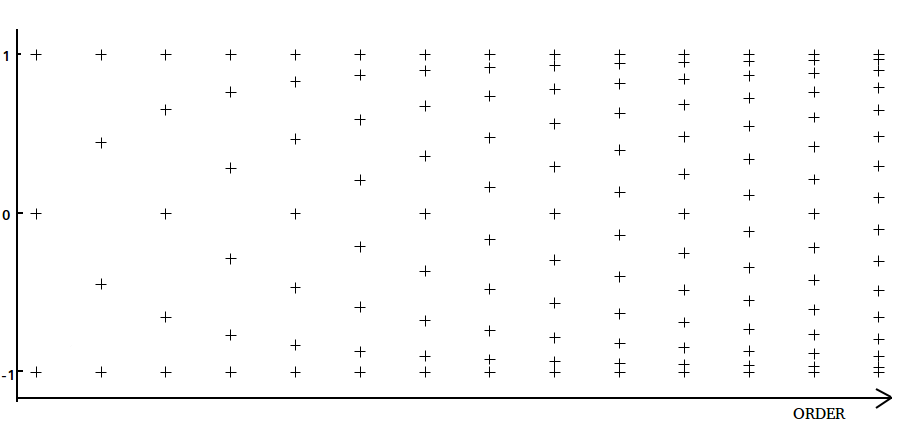
\includegraphics[width=10cm]{gauss-lobatto_points.png}
\caption{\label{GL-points} Gauss-Lobatto points for order $p=2,\dots ,15$.}
\end{figure}

\begin{figure}[h]
\centering
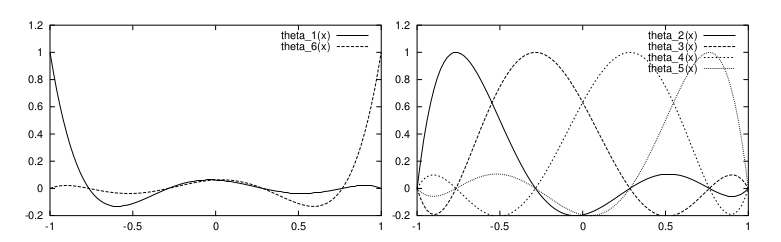
\includegraphics[width=11.5cm]{Gauss-Lobatto-Lagrange_poly.png}
\caption{\label{GLL-poly} Fifth order Gauss-Lobatto-Lagrange polynomials.}
\end{figure}


The continuous Galerkin scheme is applied, implying that, globally, for two contiguous elements $k$ and $k+1$, the polynomial $\theta_p$ in the element $k$ and the polynomial $\theta_0$ in element $k+1$, are considered as one function. This function, known as vertex function and defined in $[0,L]$, is zero in all the domain except in the element $k$ where it takes the values of $\theta_p$ and in element $k+1$ where it takes the values of $\theta_0$. On the other hand we have the bubble functions, that are defined as zero in all the domain except for on element, where they take the value of one of the polynomials $\theta_1$ to $\theta_{p-1}$. Both vertex and bubble functions are shown in Figure \ref{fig-func}.

\begin{figure}[H]
\centering
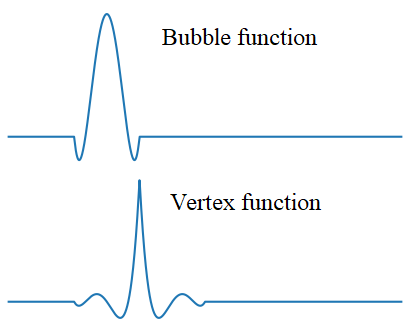
\includegraphics[width=5.5cm]{funciones_globales.png}
\caption{\label{fig-func} Descriptive scheme of vertex and bubble functions.}
\end{figure}

The set of all vertex and bubble functions compose the chosen base. For example for the case of three elements of order three, in Figure \ref{fig-ejemplofunc} all the base functions are shown. There are two special vertex functions, $\phi_0$ and $\phi_{N-1}$, they are only half of the usual vertex functions. In fact, they do not belong to the space of functions $V$, as they are not zero at $s=0$ and $s=L$. This only affects the first and last equations of the system, where the term $\mathbf{\Gamma}$ that does not vanish in the integration by parts must be added, this term is: 

\begin{equation}
\displaystyle
\mathbf{\Gamma} = \left(\ba{c} -\mathbf{F}_0 \\ 0 \\ \vdots\\ 0 \\ \mathbf{F}_{N-1}\\ \ea\right)
\end{equation}

In summary and adding some notation, this are the important aspects of the spatial discretization:

\begin{itemize}
    \item $p$ is the order of the polynomials.
    \item $n-1$ is the number of elements and $h = \frac{L}{m-1}$ is the length of each element.
    \item $N = n + (n-1)(p-1) = p(n-1) + 1$ is the number of base functions\footnote{Note that $n$ is the number of vertex functions and $(n-1)(p-1)$ is the number of bubble functions.}.
    \item $s_i = h\left( \frac{i-(i\%p)}{p} + \frac{1 + \xi_{(i \% p)}}{2} \right)$ are the discretization nodes\footnote{Here $(a\% b)$ denotes the $(a \mod b)$, and the reader should note that $\frac{i-(i\%p)}{p}$ is the element index and $\frac{1 + \xi_{(i \% p)}}{2}$ maps the quadrature nodes from $[-1,1]$ to $[0,1]$.}.
\end{itemize}

\begin{figure}[H]
	\centering
	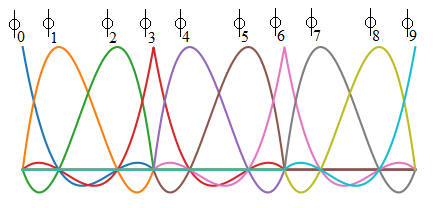
\includegraphics[width=10cm]{notation1.png}
	\caption{\label{fig-ejemplofunc} Example of base functions for three third order elements.}
\end{figure}


For the base choice, the formal formulation would be as follows.

$$\phi_i(s) = \left\{ \ba{l} 
\alpha_i(s) \quad\quad if \quad (i\% p) = 0\quad\\ 
\beta_i(s) \quad\quad else
\ea \right.$$

\vspace{1cm}

where $\alpha_i(s)$ is the vertex function:

$$\alpha_i(s) = \left\{ \ba{l}
\left\{ \ba{l}
\theta_0(2\cdot\frac{s-s_i}{h}-1)\quad if\quad s_{i}\leq s\leq s_{i+p} \\
0\qquad else \\
\ea \right\}\quad if\quad i=0 \\
\\
\left\{ \ba{l}
\theta_p(2\cdot\frac{s-s_{i-p}}{h}-1)\qquad if\quad s_{i-p}\leq s<s_{i} \\
0\qquad else \\
\ea \right\}\quad if\quad i=N-1 \\
\\
\left\{ \ba{l}
\theta_0(2\cdot\frac{s-s_{i}}{h}-1)\quad\quad if\quad s_{i}\leq s\leq s_{i+p}  \\
\theta_p(2\cdot\frac{s-s_{i-p}}{h}-1)\quad\quad if\quad s_{i-p}\leq s<s_{i}  \\
0\quad\quad else \\
\ea \right\}\quad else \\
\ea \right.$$

\vspace{1cm}

and $\beta_i(s)$ is the bubble function:

$$\beta_i(s) = \left\{ \ba{l} 
\theta_{(i\% p)}(2\cdot\frac{s-s_{p(k-1)}}{h}-1)\quad\quad if\quad s_{p\cdot k}\leq s\leq s_{p\cdot (k+1)} \\
0\quad\quad else\\
\ea \right.$$

where $k = \frac{i-(i\%p)}{p}$ is the element index. The base functions are continuous, but their derivatives are not, because of this it is necessary to take a special care when computing derivatives using these functions, and that is done in the next section.\\

\subsubsection{Derivatives and non-linear terms}

With the current basis, if the positions of the discretization nodes, $(r_0, r_1, \dots, r_{N-1})^T$, are known, the derivatives at any point of the chain can be computed with:

$$\frac{\pa^n\mathbf{r}}{\pa s^s}(s)=\sum_{i=0}^{N-1} r_i \frac{\pa^n\phi_i}{\pa s^n}(s)= \left( \frac{\pa^n\phi_0}{\pa s^n}(s), \frac{\pa^n\phi_1}{\pa s^n}(s), \dots , \frac{\pa^n\phi_{N-1}}{\pa s^n}(s) \right)\cdot \left(\ba{c} r_0 \\ r_1 \\ \vdots \\ r_{N-1} \ea\right)$$

In general, it is interesting to compute the derivatives at the discretization nodes, in matrix notation, this can be done with the following expression:

$$\displaystyle
 \left(\ba{c} \frac{\pa^n\mathbf{r}}{\pa s^n}(s_0) \\ \frac{\pa^n\mathbf{r}}{\pa s^n}(s_1) \\ \vdots \\ \frac{\pa^n\mathbf{r}}{\pa s^n}(s_{N-1}) \ea\right) =  \mathbf{D}_n \left(\ba{c} r_0 \\ r_1 \\ \vdots \\ r_{N-1} \ea\right)$$
 
where:

$$\displaystyle
\mathbf{D}_n = \left(\ba{c} \frac{\pa^n\phi_0}{\pa s^n}(s_0)\quad\quad \frac{\pa^n\phi_1}{\pa s^n}(s_0)\quad \dots \quad \frac{\pa^n\phi_{N-1}}{\pa s^n}(s_0) \\ \frac{\pa^n\phi_0}{\pa s^n}(s_1)\quad\quad \frac{\pa^n\phi_1}{\pa s^n}(s_1)\quad \dots\quad \frac{\pa^n\phi_{N-1}}{\pa s^n}(s_0) \\ \vdots\quad\quad\quad\quad\quad\quad\vdots\quad\quad\quad\quad\quad\quad\vdots\\ \frac{\pa^n\phi_0}{\pa s^n}(s_{N-1})\quad \frac{\pa^n\phi_1}{\pa s^n}(s_{N-1}) \dots \frac{\pa^n\phi_{N-1}}{\pa s^n}(s_{N-1}) \ea\right)$$

and for the points where there is a discontinuity in the derivative, the following approximation is used:

$$\displaystyle
\frac{\pa^n\phi_i}{\pa s^n}(s_j) = \frac{1}{2}\left(\frac{\pa^n\phi_i}{\pa s^n}(s_j^{-}) + \frac{\pa^n\phi_i}{\pa s^n}(s_j^{+}) \right)$$

The global derivation matrix of order $n$, $\mathbf{D}_n$ is constant in time and it is computed only once, unless the line length changes, in which case the matrix can be updated with a scalar multiplication. It can be assembled using the local derivation matrix, $\mathbf{D}_n^L$, defined as $(\mathbf{D}_n^L)_{ij}= \frac{\pa^n\theta_j}{\pa x^n}(\xi_i)$, using the following algorithm.

$$\ba{l}
\mathbf{D}_n = \mathbf{0}_{N\times N} \\
\quad \\
for \quad (k=0:n-1)\{ \\
\quad \mathbf{D}_n[ k\cdot p:(k+1)\cdot p,\quad k\cdot p:(k+1)\cdot p ] = \mathbf{D}_n[ k\cdot p:(k+1)\cdot p,\quad k\cdot p:(k+1)\cdot p ] + \mathbf{D}_n^L \\
\} \\
\quad \\
for \quad (k=1:n-1)\{ \\
\quad \mathbf{D}_n[ k\cdot p:(k+1)\cdot p,\quad : \quad ] = \mathbf{D}_n[ k\cdot p:(k+1)\cdot p,\quad : \quad ] \cdot \frac{1}{2} \\
\} \\
\\
\mathbf{D}_n = \left(\frac{2}{l}\right)^n \cdot \mathbf{D}_n
\ea$$

In this algorithm, first the global derivation matrix is initialized and then the values of the local derivation matrix are inserted in the global matrix with a first loop over all elements, as shown in Figure \ref{fig-assemble} for a case with four elements of order three. In a second loop, the rows of the matrix that relate to nodes where the base functions derivatives present discontinuities are divided by two, as shown in Figure \ref{fig-dividebytwo} (the values of the derivatives at both sides of the node were already summed in the previous loop). Finally, the full matrix is multiplied by the factor $\left(\frac{2}{l}\right)^n$, that is necessary because the chain rule of derivation is being applied with the mapping from $[-1,1]$ to $[s_k,s_{k+1}]$ at every element $k$.

\begin{figure}[H]
	\centering
	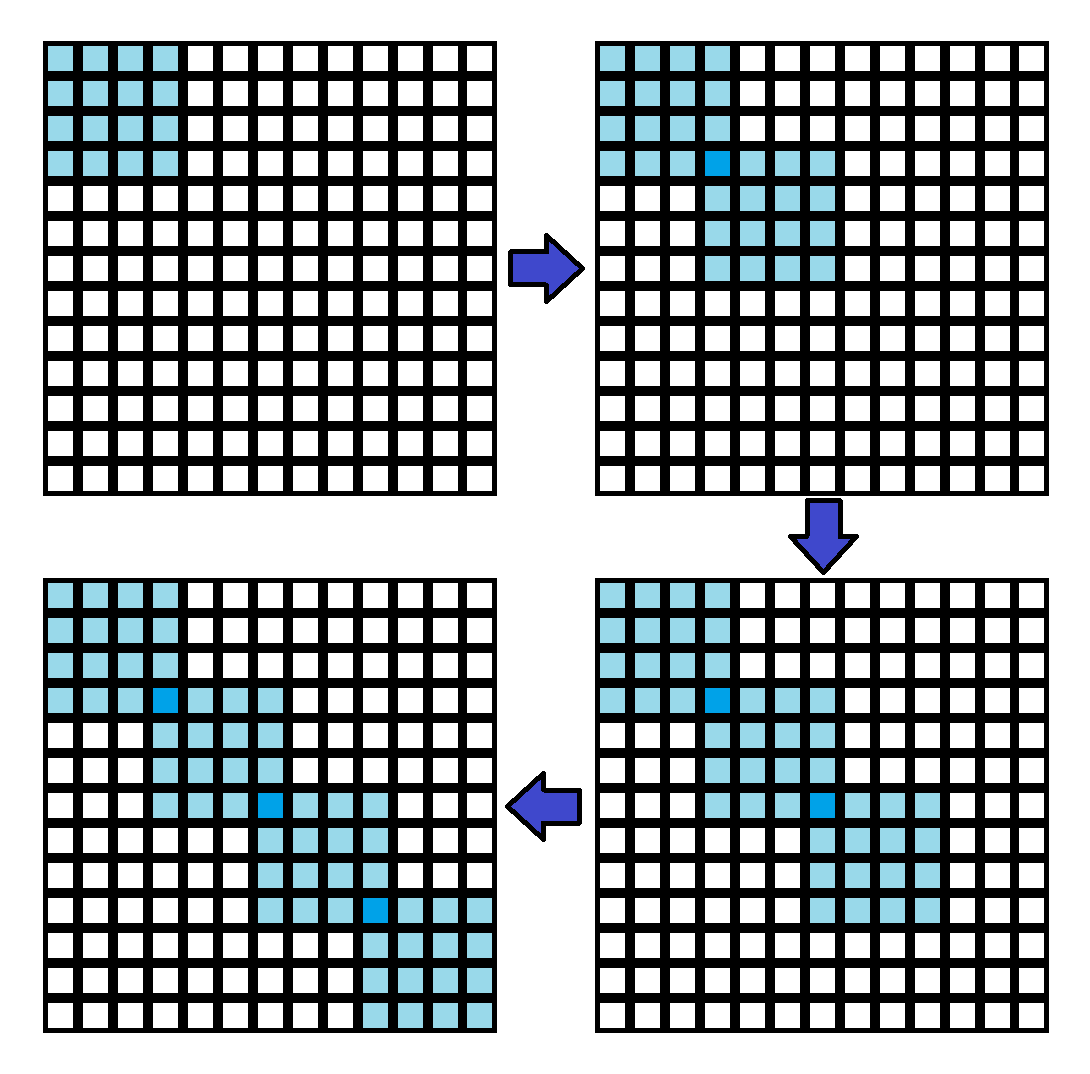
\includegraphics[width=8cm]{1_mat_MK.png}
	\caption{\label{fig-assemble} Assembling step. In the top left corner of the figure, only the first local matrix $\mathbf{D}_n^L$ has been added to the full matrix. In the dark blue elements, the values of $\mathbf{D}_n^L[0,0]$ and $\mathbf{D}_n^L[p,p]$ are being summed. }
\end{figure}

\begin{figure}[H]
	\centering
	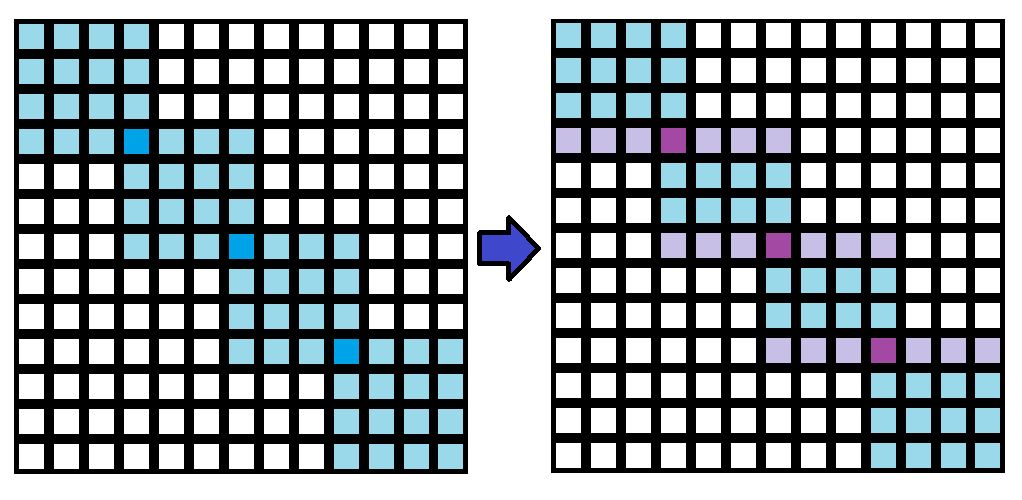
\includegraphics[width=8cm]{1_mat_D.png}
	\caption{\label{fig-dividebytwo} Discontinuity of derivatives treatment. The purple rows are divided by two to average the value of the derivative at both sides of de node.}
\end{figure}

If the line nodes velocities are known, the crossed derivatives at the nodes can also be computed easily using the global derivation matrix:

$$\left(\ba{c} \frac{\pa^n\mathbf{r}}{\pa s^n \pa t}(s_0) \\ \frac{\pa^n\mathbf{r}}{\pa s^n \pa t}(s_1) \\ \vdots \\ \frac{\pa^n\mathbf{r}}{\pa s^n \pa t}(s_{N-1}) \ea\right) =  \mathbf{D}_n \left(\ba{c} \frac{\pa r_0}{\pa t} \\ \frac{\pa r_1}{\pa t} \\ \vdots \\ \frac{\pa r_{N-1}}{\pa t} \ea\right)$$

Once all the derivatives are known, it is easy to compute all the non-linear terms that appear in the expressions of $\mathbf{F}$ and $\hat{\mathbf{f}}$:

\begin{itemize}
	\item $\mathbf{t}(s_i)=\frac{\mathbf{r}'(s_i)}{\left| \mathbf{r}'(s_i) \right|}$
    \item $e(s_i) = |\mathbf{r}'(s_i)| - 1$
    \item $\dot{e}(s_i) = \mathbf{t}(s_i)\cdot\dot{\mathbf{r}}'(s_i)$
\end{itemize}

Although directly computing second or higher order spatial derivatives is possible with this method, the error increases drastically when this is done, and it should always be avoided. For example, in this case, using the weak formulation and integration by parts, it was possible to change a product of a second order derivative with a function for a product of two first order derivatives.

Introducing first order derivatives, which also have a small error, in non-linear expressions where parameters of order up to $10^8$ appear, may produce an error that affects significantly the solution, specially when the interpolated functions are not smooth. \textbf{\textcolor{Red}{For this reason, it would be interesting to perform an analysis of the error, in order to know which is the roughest discretization required to obtain a reasonable solution.}}

\subsubsection{Integrals and system matrices}

In general, for a continuous function $f(x)$ defined in $[-1,1]$, Gauss-Lobatto quadrature of order $p$ can be applied to compute the integral:

$$\int_{-1}^{1} f(x) dx = \sum_{i=0}^{p}\omega_i\cdot f(\xi_{i,p-1}) + E$$

where $E$ is the error of the quadrature rule and the Gauss-Lobatto weights $\{\omega_i\}$ and nodes $\{\xi_{i,p-1}\}$ can be computed with the method detailed in Karniadakis \cite{karniadakis} book, page 61. If $f(x)$ is a polynomial of order less or equal to $2\cdot p-1$, then the quadrature is exact ($E=0$).\\

If a discretization of order $p$ is chosen for the studied line, a quadrature rule of order at least $p+1$ is necessary to evaluate exactly\footnote{If the order of the discretization is $p$, the order of the product $\phi_i\phi_j$ is $2\cdot p$, and a quadrature of order $p$ would be insufficient to compute the integral of this product exactly.} the integrals that appear in Equation \ref{matrices-integrals}. In each element of the discretization, the same local function base is used, and then, the elementary matrices can be used to assemble the full matrices. For element $k$:

$$\mathbf{M}_{ij}^{(k)} = \int_{s_{p\cdot k}}^{s_{p\cdot (k+1)}} \theta_i(\frac{2}{h}(s-s_{p\cdot k})-1) \cdot\theta_j(\frac{2}{h}(s-s_{p\cdot k})-1)ds = \left(\frac{h}{2}\right)\cdot\int_{-1}^{1} \theta_i(x)\cdot\theta_j(x) dx $$

$$\ba{r} \mathbf{K}_{ij}^{*(k)} = \int_{s_{p\cdot k}}^{s_{p\cdot (k+1)}} \left(\theta_i(\frac{2}{h}(s-s_{p\cdot k})-1)\right) ' \cdot\theta_j(\frac{2}{h}(s-s_{p\cdot k})-1)ds = \\
\\
=\int_{s_{p\cdot k}}^{s_{p\cdot (k+1)}} \left(\frac{2}{h}\right)\cdot\theta_i'(\frac{2}{h}(s-s_{p\cdot k})-1) \cdot\theta_j(\frac{2}{h}(s-s_{p\cdot k})-1)ds = \\
\\
=\left(\frac{h}{2}\right)\cdot\int_{-1}^{1} \left(\frac{2}{h}\right)\cdot\theta_i'(x)\cdot\theta_j(x) dx = \int_{-1}^{1} \theta_i'(x)\cdot\theta_j(x) dx \ea$$


These elementary matrices are the same for every element, we define constant elementary matrices $\mathbf{M}^{(e)}$ and $\mathbf{K}^{*(e)}$ as $\mathbf{M}_{ij}^{(e)} = \left(\frac{h}{2}\right)\cdot\int_{-1}^{1} \theta_i(x)\cdot\theta_j(x) dx$ and $\mathbf{K}_{ij}^{*(e)} = \int_{-1}^{1} \theta_i'(x)\cdot\theta_j(x) dx$. The following algorithm is used for assembling of the full matrices:

$$
\ba{l}
\mathbf{M} = \mathbf{0}_{N\times N} \\
\mathbf{K}^* = \mathbf{0}_{N\times N} \\
\quad \\
for \quad (k=0:n-2)\{ \\
\quad \mathbf{M}[ k\cdot p:(k+1)\cdot p+1,\quad k\cdot p:(k+1)\cdot p+1 ] =  \\
\quad \quad \quad =\mathbf{M}[ k\cdot p:(k+1)\cdot p+1,\quad k\cdot p:(k+1)\cdot p+1 ] + \mathbf{M}^{(e)} \\
\quad \mathbf{K}^*[ k\cdot p:(k+1)\cdot p+1,\quad k\cdot p:(k+1)\cdot p+1 ] =  \\
\quad \quad \quad =\mathbf{K}^*[ k\cdot p:(k+1)\cdot p+1,\quad k\cdot p:(k+1)\cdot p+1 ] + \mathbf{K}^{*(e)} \\
\} \\
\ea
$$

This algorithm is the same as the one used for the derivation matrix in Figure \ref{fig-assemble}, but without dividing by two, since there are no discontinuities in this case. Also, the elementary matrices are computed using Gauss-Lobatto Gaussian quadrature with the following algorithm:

$$
\ba{l}
\mathbf{M}^{(e)} = \mathbf{0}_{N\times N} \\
\mathbf{K}^{*(e)} = \mathbf{0}_{N\times N} \\
for \quad (i=0:p)\{ \\
\quad for \quad (j=0:p)\{ \\
\quad \quad for \quad (k=0:p+1)\{ \\
\quad \quad \quad \mathbf{M}^{(e)}[i,j] = \mathbf{M}^{(e)}[i,j] +  \left(\frac{h}{2}\right)\cdot\omega_k\cdot\theta_i(\xi_{k,p})\cdot\theta_j(\xi_{k,p})\\
\quad \quad \quad \mathbf{K}^{*(e)}[i,j] = \mathbf{K}^{*(e)}[i,j] +  \omega_k\cdot\theta'_i(\xi_{k,p})\cdot\theta_j(\xi_{k,p})\\
\quad \quad \} \\
\quad \} \\
\} \\
\ea
$$

In this algorithm there are three nested loops, the first one over the matrix rows, the second one over the matrix columns and the last one is over the quadrature nodes. The system matrices are constant in time and they are computed only once, unless for the matrix $\mathbf{M}$, and only if the line length changes, in which case the matrix can be updated with a scalar multiplication.\\

Recall that the purpose of this whole section was to compute a matrix $\mathbf{A}$ and a vector $\mathbf{B}$ such that:

$$\left(\ba{c} \mathbf{v} \\ \mathbf{a} \ea\right) = \frac{\pa\mathbf{u}}{\pa t} = f(\mathbf{u}, t) = f(\left(\ba{c} \mathbf{r} \\ \mathbf{v} \ea\right), t) = \left(\ba{c} \mathbf{v} \\ \mathbf{A}^{-1}\cdot\mathbf{B} \ea\right)$$

So far, the result is$$\mathbf{A} = \mathbf{M}$$and$$\mathbf{B} = -\mathbf{K}^*\cdot\mathbf{F}+\mathbf{M}\cdot\hat{\mathbf{f}}+\mathbf{\Gamma}$$

where the terms $\mathbf{M}$, $\mathbf{K}^*$, $\mathbf{F}$ and $\hat{\mathbf{f}}$ have been described in detail.\\ \\

Note that the final expression for computing the acceleration at the nodes of the chain is the system $\mathbf{M} \cdot \mathbf{a} =-\mathbf{K}^*\cdot\mathbf{F}+\mathbf{M}\cdot\hat{\mathbf{f}}(\mathbf{a})+\mathbf{\Gamma}$, where $\hat{\mathbf{f}}$ depends on $\mathbf{a}$ because the added mass forces are part of the external force. This problem is solved using an iterative method where the following algorithm is followed, where "tol" is the tolerance of the iterative method and "nIterMax" is the maximum number of iterations, introduced to limit the computational cost.

\begin{equation}
\nonumber
\ba{l} \text{set }\mathbf{a}^0\text{ as the acceleration at previous time-step}\\
\text{solve   }\mathbf{M} \cdot \mathbf{a}^{1} =-\mathbf{K}^*\cdot\mathbf{F}+\mathbf{M}\cdot\hat{\mathbf{f}}(\mathbf{a}^{0})+\mathbf{\Gamma}\\
k = 1\\
\\
while \quad ((||a^{k}-a^{k-1}||>\text{tol})\text{  \&  }(k<\text{nIterMax}))\{ \\
\quad \text{solve   }\mathbf{M} \cdot \mathbf{a}^{k+1} =-\mathbf{K}^*\cdot\mathbf{F}+\mathbf{M}\cdot\hat{\mathbf{f}}(\mathbf{a}^{k})+\mathbf{\Gamma}\\
\quad k = k + 1\\
\}\\
\mathbf{a} = \mathbf{a}^{k}\\
\ea 
\end{equation}

The problem is not completely solved yet. First, it is necessary to describe how to impose the boundary conditions and the initial condition. This is done in the following section.

\subsection{Boundary conditions}

Once the matrix $\mathbf{A}$ and the vector $\mathbf{B}$ in Equation \ref{system-function} are computed, it is necessary to modify them before solving the linear system in order to impose the boundary conditions. In this section, it is shown how to do this for the different options considered.

\subsubsection{Anchor, fairlead or actuator conditions}

When the line is connected to an anchor, a floating body fairlead or a lab actuator, the position, velocity and acceleration of that point of the line are known, and must be imposed. To do so, for computing the internal and external forces vectors, which depend on the position and the velocity of the line, the boundary data is considered in the calculations. Then, before solving the system, first row, last row or both rows of the system matrix are set to zero, except for the element in the diagonal, and in the forces vector the first row, the last row or both rows are changed to the acceleration that the boundary condition imposes. This is shown in Figure \ref{fig-BC1} for a case with four elements of order three where the movements of the line are both of its ends are imposed.

\begin{figure}[H]
	\centering
	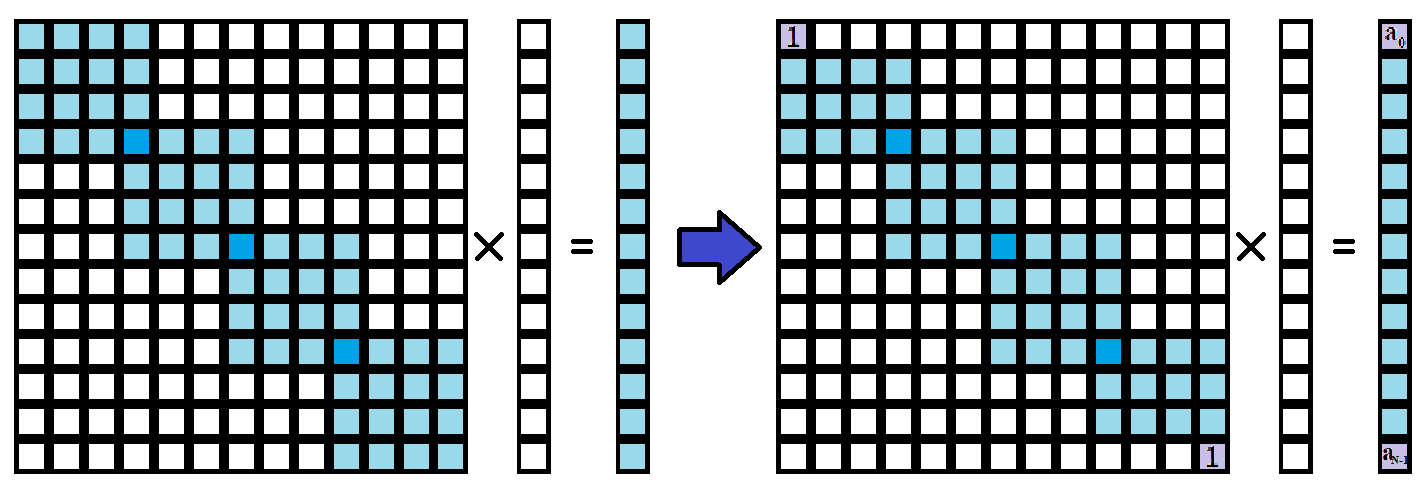
\includegraphics[width=14cm]{BoundaryConditions.png}
	\caption{\label{fig-BC1} Boundary conditions modifications on the system.}
\end{figure}

Formally, this changes are expressed with the following pseudo-code:

\begin{equation}
\nonumber
\ba{l} \mathbf{A} = \mathbf{M}\\
\mathbf{A}[0,0] = 1\\
\mathbf{A}[0,1:N-1] = 0\\
\mathbf{A}[N-1,N-1] = 1\\
\mathbf{A}[N-1,0:N-2] = 0\\
\\
\mathbf{B} = -\mathbf{K}^*\cdot\mathbf{F}+\mathbf{M}\cdot\hat{\mathbf{f}}+\mathbf{\Gamma}\\
\mathbf{B}[0,:] = \hat{\mathbf{a}}_0\\
\mathbf{B}[N-1,:] = \hat{\mathbf{a}}_{N-1}\\
\ea 
\end{equation}

where $\hat{\mathbf{a}}_0$ and $\hat{\mathbf{a}}_{N-1}$ are the accelerations imposed at nodes $0$ and $N-1$ respectively.\\


\subsubsection{Multi-line joint conditions}

An important feature of a line simulation software is to be able study the case where more than one line are connected to one point. An example of this situation is the crowfoot or delta mooring system, where there are two fairleads, one anchor, and three lines that join these three points to a common one, as shown in Figure \ref{fig-crowfoot}.

\begin{figure}[H]
	\centering
	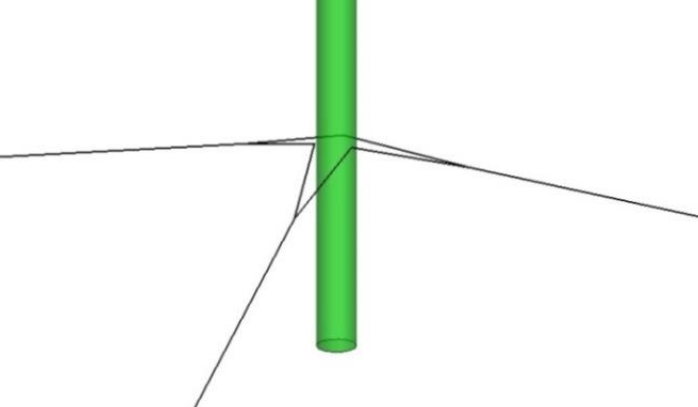
\includegraphics[width=8cm]{crowfoot.PNG}
	\caption{\label{fig-crowfoot} Crowfoot or delta mooring system.}
\end{figure}

Let there be a set of $n$ lines converging to the same point, where $\{(\rho_0)_i\}$ are the linear weights of the different lines. In order to apply the joint boundary condition, first, the averages of the positions and the velocities of all the nodes that converge to the joint are imposed to those nodes, before computing the internal and external forces vectors. After that, the lines systems are solved without making any change to the equations of the nodes that are connected to the joint. Then, once the accelerations of all the nodes connected to the joint, $\{\hat{\mathbf{a}}_i\}$, are known, the acceleration of the joint, $\mathbf{a}_J$ is computed as:

$$\mathbf{a}_J = \frac{\sum_{i = 1}^n\left[(\rho_0)_i\cdot\hat{\mathbf{a}}_i\right]}{\sum_{i = 1}^n(\rho_0)_i}$$

Finally, this acceleration is imposed to all the nodes that converge to the joint.

\subsubsection{Winch condition}

Other important feature is to be able to simulate lines connected to winches, that may vary their length depending on the momentum applied with the winches engines, $M$, the properties of the winches (radius $R$ and mass $m$) and the tension $T$ of the lines at the winches. Figure \ref{fig-winche} shows the scheme of a winch.\\

\begin{figure}[H]
	\centering
	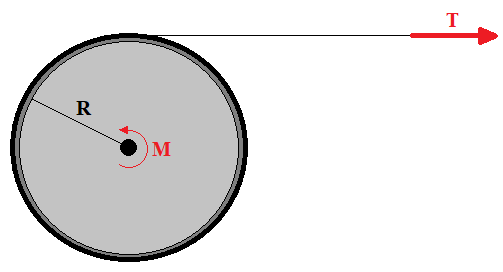
\includegraphics[width=8cm]{winch.PNG}
	\caption{\label{fig-winche} Winch scheme.}
\end{figure}

\vspace{1cm}

There are two aspects that we have to consider when there is a winch at the end of a line. The first one is how to compute how the winch rotates, and the second one is to compute how the winch rotation modifies the line length, and how the length variation affects the equations of the line.

In order to simulate the rotation of the winch, the Newton equation is applied in Equation \ref{eq-winch}.

\bean I\cdot \alpha = T\cdot r - M \label{eq-winch}\eean

The left side of Equation \ref{eq-winch} is the product of moment of inertia of the winch with the angular acceleration of the winch for rotations around the winch's axis. If the winch is considered to be a cylinder, the moment of inertia of the winch is $I=\frac{1}{2}\cdot m\cdot R^2$. The right side of the equation is the sum of the momentum that is applied to the winch, first the momentum that the line applies, considering that the radius of the winch and the tension of the line are perpendicular, and finally the momentum that the winch's engine applies. The signs are chosen some how that if the angle of rotation of the winch is positive, the line length increases, and if the winch's engine applies a positive momentum strong enough, the line length decreases.

Winch's time evolution is then described by the following initial value problem:

$$\left\{ \ba{l} \frac{\pa\mathbf{u}}{\pa t} = f(t) \\  \\ \mathbf{u}(0) = \mathbf{u}_0 \ea \right.$$

With $f$ being the ODE function, $\mathbf{u}_0$ known initial condition, and $\mathbf{u}$ the unknown. In this case the unknown will be: 

$$\mathbf{u}=\left(\ba{c} \theta \\ \omega \ea\right) $$

where $\theta$ and $\omega$ are, respectively, the rotation and the angular velocity of the winch. The initial condition will be considered as zero:

$$\mathbf{u}_0=\left(\ba{c} 0 \\ 0 \ea\right) $$

and the ODE function is:

\bean
\left(\ba{c} \omega \\ \alpha \ea\right) = \frac{\pa\mathbf{u}}{\pa t} = f(t) = \left(\ba{c} \omega \\ I^{-1}\cdot(T\cdot r - M) \ea\right)
\label{system-function-winch}
\eean

This ODE is integrated together with the line ODE, and the coupling between the winch and the line consists in that the line tension is used in the winch ODE and the winch rotation is used un the line ODE. This is because the line length is dependent on the winch rotation as it is shown in Equation \ref{eq-winchL}.

\bean L = L_0 + \theta\cdot R \label{eq-winchL}\eean

where $L$ is the line length, $L_0$ is the initial line length, and $theta$ and $R$, are respectively and as mentioned before, the winch rotation and radius. When the line length changes, instead of using the global derivation matrices $\mathbf{D}_n$ and the mass matrix $\mathbf{M}$ described in the previous section and used in the line ODE, the following matrices must be used instead:

$$\mathbf{D}_n \Rightarrow \left(\frac{L_0}{L}\right)^n\cdot\mathbf{D}_n$$
$$\mathbf{M} \Rightarrow \left(\frac{L}{L_0}\right)\cdot\mathbf{M}$$

With this, all the studied boundary conditions are already described, and only the last step is needed: the computation of the initial condition for all the line nodes.

\vspace{1cm}

\subsection{Initial condition}

For the initial condition, in general, a quasi-static (QS) method is used to find the positions of the line nodes. The velocity and acceleration of these nodes are considered as zero for the initial conditions. The QS method used is based in \cite{faltinsen}, an in this section a description of the method is presented. \\ \\

The QS method ignores the dynamic effects on the line as inertia, friction, damping, or added mass and considers the line to be contained in a plane. The variables used for the QS method are:\\ \\

\begin{tabular}{ll}
	$\rho_w$ & water density, \\ 
	$A$ & line section \\
	$\rho_0$ & line mass per unit of length, \\
	$\mathbf{g}$ & gravity acceleration vector, \\
	$x_{F}$ & horizontal span between line ends, \\
	$z_{F}$ & vertical span between line ends, \\
	$H_{F}$ & horizontal tension at line's top support (usually the fairlead), \\
	$V_{F}$ & vertical tension at line's top support, \\
	$H_{A}$ & horizontal tension at line's bottom support (usually the anchor), \\
	$V_{A}$ & vertical tension at line's bottom support, \\
	$\omega = (\rho_0-rho_w\cdot A)*g$ & line's underwater weight, \\
	$L$ & line length, \\
	$L_B$ & line length lying over the sea floor, \\
	$E$ & line Young's modulus and \\
	$C_{B}$ & line-ground friction coefficient. \\ \\
\end{tabular}

Usually, the horizontal and vertical spans $x_{F}$ and $z_{F}$ are known and the unknowns are the tension values at both ends of the line. 

\vspace{1cm}
On literature, the following expressions are found for the horizontal an vertical spans in terms of the top support tension:\\

\hspace{1cm}\textbf{If the line does not lie on the sea floor} ($L_B = L - \frac{V_F}{\omega} \leq 0$):

\begin{equation}
\nonumber
x(H_{F},V_{F}) = \frac{H_{F}}{\om} \left[ \ln \left( \frac{V_{F}}{H_{F}} + \sqrt{1+\left( \frac{V_{F}}{H_{F}} \right)^{2} } \right) - \ln \left( \frac{V_{F}-\om L}{H_{F}} + \sqrt{1+\left( \frac{V_{F}-\om L}{H_{F}} \right)^{2} } \right) \right] + \frac{H_{F} L}{EA}
\end{equation}

\begin{equation}
\nonumber
z(H_{F},V_{F}) = \frac{H_{F}}{\om} \left[\sqrt{1+\left( \frac{V_{F}}{H_{F}} \right)^{2} } - \sqrt{1+\left( \frac{V_{F}-\om L}{H_{F}} \right)^{2} } \right] + \frac{1}{EA} \left( V_{F} L - \frac{\om L^{2}}{2}\right)
\end{equation}

\vspace{1cm}
\hspace{1cm}\textbf{If part of the line lies on the sea floor}\footnote{In this case, there is a "max" term, which differentiates if there is horizontal tension in the anchor or not. This should be considered as two separate cases for the Newton-Raphson method in order to compute the Jacobean matrix derivatives.} ($L_B = L - \frac{V_F}{\omega} > 0$):

\begin{multline}
\nonumber
x(H_{F},V_{F}) = L - \frac{V_{F}}{\om} + \frac{H_{F}}{\om} \ln \left( \frac{V_{F}}{H_{F}} + \sqrt{1+\left( \frac{V_{F}}{H_{F}} \right)^{2} } \right)  + \frac{H_{F} L}{EA}+ \\
+ \frac{C_{B} \om}{2 EA} \left[ - \left( L - \frac{V_{F}}{\om} \right)^{2} + \left( L - \frac{V_{F}}{\om}  - \frac{H_{F}}{C_{B}\om}\right) \max \left( L - \frac{V_{F}}{\om} - \frac{H_{F}}{C_{B}\om},0 \right)
\right]
\end{multline}

\begin{equation}
\nonumber
z(H_{F},V_{F}) = \frac{H_{F}}{\om} \left[\sqrt{1+\left( \frac{V_{F}}{H_{F}} \right)^{2} } - 1 \right]
+ \frac{1}{EA} \left( V_{F} L - \frac{\om L^{2}}{2}\right) 
\end{equation}

\vspace{1cm}

Finding the pair $(H_{F},V_{F})$ that yields the desired spans implies solving a non-linear system of equations, and this is done using a Newton-Raphson method. To do so, the function $\mathbf{F}(H_{F},V_{F})$ is the defined as:

$$\mathbf{F}(H_{F},V_{F}) = \left(\ba{c} x(H_{F},V_{F}) - x_{F} \\ z(H_{F},V_{F}) - z_{F} \ea\right)$$

in a way that the solution of the equation $\mathbf{F}(H_{F},V_{F})=0$ is the solution of the non-linear system. Let $\mathbf{J}$ be the Jacobean matrix of $\mathbf{F}$. Let the unknown be expressed as $\mathbf{x} = (H_{F}, V_{F})^T$. Let the initial guess be:

$$ \mathbf{x}^0 = \left(\left| \frac{\om x_{F}}{2 \lambda_{0}}\right|, \frac{\om}{2} \left[\frac{z_{F}}{\tanh(\lambda_{0})} + L \right]\right)^T $$

where:

$$ \lambda_{0} = \left\{ \ba{ll} 
10^{6}                                                 & \text{for } x_{F} = 0 \\ 
0.2                                                    & \text{for } \sqrt{x_{F}^2+z_{F}^2} \geq L \\
\sqrt{3 \left( \frac{L^2-z_{F}^2}{x_{F}^2} - 1 \right)} & \text{otherwise.} \ea \right. $$

Then the solution is obtained updating the estimation of the solution with the expression:

$$\mathbf{x}^{k+1} = \mathbf{x}^{k} - \mathbf{J}^{-1}(\mathbf{x}^{k})\cdot\mathbf{F}(\mathbf{x}^{k})$$

until the convergence criteria $||\mathbf{x}^{k+1} - \mathbf{x}^{k}||< \text{tol}$ is met, where "tol" is the tolerance, or until the maximum number of iterations is reached.


Once the tension at the top support is obtained, the tension at the bottom can be easily computed with:\\

\hspace{1cm}\textbf{If the line does not lie on the sea floor}:

\begin{equation}
\nonumber
H_{A} = H_{F} \qquad V_{A} = V_{F} - \om L
\end{equation}

\vspace{1cm}
\hspace{1cm}\textbf{If part of the line lies on the sea floor}:

\begin{equation}
\nonumber
H_{A} = \max(H_{F} - C_{B} \om L_{B},0) \qquad V_{A} = 0
\end{equation}


\vspace{1cm}

Finally, the position and tension of any point of the line can be computed with the following expressions:


\hspace{1cm}\textbf{If the line does not lie on the sea floor}:

\bean
\nonumber
x(s) = \frac{H_{F}}{\om} \left[ \ln \left( \frac{V_{A} + \om s}{H_{F}} + \sqrt{1+\left( \frac{V_{A}+\om s}{H_{F}} \right)^{2} } \right) - \ln \left( \frac{V_{A}-\om L}{H_{F}} + \sqrt{1+\left( \frac{V_{A}-\om L}{H_{F}} \right)^{2} } \right) \right] + \frac{H_{F} s}{EA} 
\eean

\bean
\nonumber
z(s) = \frac{H_{F}}{\om} \left[\sqrt{1+\left( \frac{V_{A}+\om s}{H_{F}} \right)^{2} } - \sqrt{1+\left( \frac{V_{A}}{H_{F}} \right)^{2} } \right] + \frac{1}{EA} \left( V_{A} s - \frac{\om s^{2}}{2}\right)
\eean

\bean
\nonumber
T_{e}(s) = \sqrt{H_{F}^{2} + (V_{A} + \om s)^{2}}
\eean

\vspace{1cm}
\hspace{1cm}\textbf{If part of the line lies on the sea floor}:

\bean
\nonumber
\hspace{-0.5cm} x(s) =  \left\{ \ba{cl} s, & \hspace{-0.25cm} 0 \leq s \leq L_{B} - \frac{H_{F}}{C_{B} \om} \\ & \\
s + \frac{C_{B} \om}{2EA} \left[ \ba{lr} s^{2} - 2 \left(L_{B} - \frac{H_{F}}{C_{B} \om} \right) s \\+\left(L_{B} - \frac{H_{F}}{C_{B} \om}  \right)  \max\left(L_{B} - \frac{H_{F}}{C_{B} \om} ,0\right) \ea \right] 
, & \hspace{-0.25cm} L_{B} - \frac{H_{F}}{C_{B} \om}   \leq s \leq L_{B}\\ & \\
\ba{lr}L_{B} + \frac{H_{F}}{\om} \ln \left[ \frac{\om(s-L_{B})}{H_{F}} + \sqrt{1+\left(\frac{\om(s-L_{B})}{H_{F}} \right)^{2}} \right] + \frac{H_{F}s}{EA} \\
+ \frac{C_{B} \om}{2EA} \left[ -L_{B}^{2} + \left(L_{B} - \frac{H_{F}}{C_{B} \om}  \right)  \max\left(L_{B} - \frac{H_{F}}{C_{B} \om} ,0\right) \right]\ea 
, & \hspace{-0.25cm} L_{B}   \leq s \leq L
\ea \right.
\eean

\bean
\nonumber
z(s) =  \left\{ \ba{cl} 0, & 0 \leq s \leq L_{B} \\ & \\
\frac{H_{F}}{\om} \left[\sqrt{1+\left( \frac{V_{F}}{H_{F}} \right)^{2} } - 1 \right] + \frac{1}{EA} \left( V_{F} L - \frac{\om L^{2}}{2}\right) , & L_{B}  \leq s \leq L \ea \right.
\eean

\bean
\nonumber
T_{e}(s) = \left\{ \ba{cl} \max(H_{F} + C_{B} \om (s - L_{B}),0), & 0 \leq s \leq L_{B} \\ & \\
\sqrt{H_{F}^{2} + (\om (s-L_{B}))^{2}}, & L_{B}  \leq s \leq L \ea \right.
\eean

This is enough to compute the initial condition for most of the cases, but there are some exceptions in which the iterative method does not converge, or when the line system is not valid for the quasi-static approximation, for example, when there is a crowfoot joint or when the line is too tense. In this cases, an approximated initial condition will be used, considering the lines straight between their ends, and a previous simulation must be done to find the equilibrium state, which will be considered as the initial condition for other simulations.

Also if the case of study does not require a really precise mooring or towing lines simulation, or needs to be really fast, the QS method can be coupled with the floating bodies to run time evolution simulation.

\clearpage
%%%%%%%%%%%%%%%%%%%%%%%%%%%%%%%%%%%%%%%%%%%%%%%%%%%%%%%%%%%%%%%%%%%%%%%%%%%
%   Wind turbine
%%%%%%%%%%%%%%%%%%%%%%%%%%%%%%%%%%%%%%%%%%%%%%%%%%%%%%%%%%%%%%%%%%%%%%%%%%%
\section{Wind turbine}
To be developed.


%%%%%%%%%%%%%%%%%%%%%%%%%%%%%%%%%%%%%%%%%%%%%%%%%%%%%%%%%%%%%%%%%%%%%%%%%%%
%   Oscillating water columns
%%%%%%%%%%%%%%%%%%%%%%%%%%%%%%%%%%%%%%%%%%%%%%%%%%%%%%%%%%%%%%%%%%%%%%%%%%%
\section{Oscillating water columns}
To be developed.


%%%%%%%%%%%%%%%%%%%%%%%%%%%%%%%%%%%%%%%%%%%%%%%%%%%%%%%%%%%%%%%%%%%%%%%%%%%
%   Mechanical systems
%%%%%%%%%%%%%%%%%%%%%%%%%%%%%%%%%%%%%%%%%%%%%%%%%%%%%%%%%%%%%%%%%%%%%%%%%%%
\section{Mechanical systems}
(Alvaro) (6 DOF springs)


%%%%%%%%%%%%%%%%%%%%%%%%%%%%%%%%%%%%%%%%%%%%%%%%%%%%%%%%%%%%%%%%%%%%%%%%%%%
%   Time integration
%%%%%%%%%%%%%%%%%%%%%%%%%%%%%%%%%%%%%%%%%%%%%%%%%%%%%%%%%%%%%%%%%%%%%%%%%%%
\section{Time integration}
(Alvaro) (BDF2 with variable step)


%%%%%%%%%%%%%%%%%%%%%%%%%%%%%%%%%%%%%%%%%%%%%%%%%%%%%%%%%%%%%%%%%%%%%%%%%%%
%   Coupling
%%%%%%%%%%%%%%%%%%%%%%%%%%%%%%%%%%%%%%%%%%%%%%%%%%%%%%%%%%%%%%%%%%%%%%%%%%%
\section{Coupling}
(Alvaro) (Weak coupling)



\clearpage

\bibliographystyle{empty} %%%%%%%%%%%%%%%%%%%%%%%%%%%%%%%%%%%%%%%%%%%%%%%%%%%%%%%%%%%%%%%%%%%%%%%%%%%%%%
\begin{thebibliography}{9}
	
\bibitem{ODEPACK}
A. C. Hindmarsh, ODEPACK, A Systematized Collection of ODE Solver, Editors:Stepleman, Carver, Peskin, Ames and Vichnevetsky: IMACS Transactions on Scientific Computation, 1983.

\bibitem{karniadakis}
G. E. Karniadakis, Spectral/hp Element Methods for computational Fluid Dynamics. Second Edition. Oxford science Publications, 2004.

\bibitem{azcona}
J. Azcona, Computational and Experimental Modelling of Mooring Lines Dynamics for Offshore Floating Wind Turbines. UPM. 2015

\bibitem{ref-drag}
J. N. Newman, Marine Hydrodynamics, The Massachusetts Institute of Technology, 1977

\bibitem{Palm-2017} 
J. Palm, C. Eskilsson and L. Bergdahl. An hp-adaptive discontinuous Galerkin method for modelling snap loads in mooring cables. Ocean Engineering, 144: 266-276, 2017.

\bibitem{Aamo-2000}
O.M. Aamo and T.I. Fossen. Finite element modelling of mooring lines. Mathematics and Computers in Simulation, 53(4-6):415 – 422, 2000.

\bibitem{faltinsen}
O.M. Faltinsen, Sea loads on ships and offshore structures.Cambridge ocean technology series. 1999

\bibitem{Hall-2015}
M. Hall and A. Goupee. Validation of a lumped-mass mooring line model with DeepCwind semisubmersible model test data. Ocean Engineering,104:590 – 603, 2015.

\bibitem{torsion}
M. R. Escalante, M.B. Rosales, R. Sampaio and T. Ritto, Reduced order model of a 3D cable using proper orthogonal decomposition. Mec. Comp.. 30. 1143-1158. 2011

\bibitem{quintela}
P. Est\'evez. Matemáticas en ingeniería con MATLAB (Vol. 3). Universidad de Santiago de Compostela. 2001


\end{thebibliography}


\end{document}